\documentclass[twocolumn,11pt]{jarticle}
\usepackage{geometry}
\usepackage{amsmath}
\usepackage{latexsym}
\usepackage{ascmac}
\usepackage{fancyhdr}
\usepackage{subcaption}
\usepackage[dvipdfmx]{graphicx}
\graphicspath{ {math-images2/} }
\usepackage[dvipdfmx]{color}
\usepackage{overpic}
\usepackage[dvipdfmx,%
 bookmarks=true,%
 bookmarksnumbered=true,%
 colorlinks=true,%
 linkcolor=blue,%
 setpagesize=false,%
 pdftitle={数学の基礎訓練II},%
 pdfauthor={西井淳},%
 pdfsubject={数学の基礎訓練},%
 pdfkeywords={数学;微分;積分;微分方程式}]{hyperref}
\usepackage{pxjahyper}%hyperrefの不具合対応
\usepackage{makeidx} %索引
%\usepackage[extra]{mymath}
%\usepackage[answer]{mymath}
\usepackage{mymath}
\makeindex

\geometry{body={178mm,242mm},columnsep=8mm}

\begin{document}

\pagestyle{empty}
\twocolumn[
%\vspace{-0.8cm}
\noindent
\rule{\linewidth}{0.5pt}
\begin{center}
{\Huge\gtfamily 数学の基礎訓練II\\\vspace{0.3cm}
\LARGE〜微積分の基本〜}
\end{center}
%\vspace{-0.6cm}
\begin{flushright}
\today 版\quad 西井 淳
\\
\rule{\linewidth}{0.5pt}
\end{flushright}
]
{\small\tableofcontents}
\newpage
% \rule{0pt}{10cm}
% \newpage

\setcounter{page}{1}
\pagestyle{fancy}

\section{微分}

\subsection{極限}

\nquestion
以下の極限を求めなさい。必ずグラフを描いて考えること
\answer{
(\ref{litem:(x->+0)1/x}) $\infty$~
(\ref{litem:(x->-0)1/x}) $-\infty$~
(\ref{litem:(x->0)1/x}) 極限値無し~
(\ref{litem:(x->infty)1/x}) $0$~
(\ref{litem:(x->-infty)1/x}) $0$~
(\ref{litem:(x->2+0)1/x-2}) $\infty$~
(\ref{litem:(x->2-0)1/x-2}) $-\infty$~
(\ref{litem:(x->+0)|x|/x}) $1$~
(\ref{litem:(x->-0)|x|/x}) $-1$~
(\ref{litem:(x->infty)e^x}) $\infty$
(\ref{litem:(x->-infty)e^x}) $0$~
(\ref{litem:(x->infty)e^-x}) $0$~
(\ref{litem:(x->-infty)e^-x}) $\infty$
}。
\begin{enumerate}
\item \label{litem:(x->+0)1/x}$\displaystyle\lim_{x\to+0}\frac{1}{x}$
\item \label{litem:(x->-0)1/x}$\displaystyle\lim_{x\to-0}\frac{1}{x}$
\item \label{litem:(x->0)1/x}$\displaystyle\lim_{x\to 0}\frac{1}{x}$
\item \label{litem:(x->infty)1/x}$\displaystyle\lim_{x\to\infty}\frac{1}{x}$
\item \label{litem:(x->-infty)1/x}$\displaystyle\lim_{x\to-\infty}\frac{1}{x}$
\item \label{litem:(x->2+0)1/x-2}$\displaystyle\lim_{x\to 2+0}\frac{1}{x-2}$
\item \label{litem:(x->2-0)1/x-2}$\displaystyle\lim_{x\to 2-0}\frac{1}{x-2}$
\item \label{litem:(x->+0)|x|/x}$\displaystyle\lim_{x\to+0}\frac{|x|}{x}$
\item \label{litem:(x->-0)|x|/x}$\displaystyle\lim_{x\to-0}\frac{|x|}{x}$
\item \label{litem:(x->infty)e^x}$\displaystyle\lim_{x\to\infty}e^x$
\item \label{litem:(x->-infty)e^x}$\displaystyle\lim_{x\to-\infty}e^x$
\item \label{litem:(x->infty)e^-x}$\displaystyle\lim_{x\to\infty}e^{-x}$
\item \label{litem:(x->-infty)e^-x}$\displaystyle\lim_{x\to-\infty}e^{-x}$
\end{enumerate}

\nquestion
以下の極限値を求めなさい
\answer{
(\ref{litem:(x->0)0/x}) $0$~
(\ref{litem:(x->0)x/0}) 値無し~
(\ref{litem:1/ex+1}) 1~
(\ref{litem:ex-e-x/ex+e-x}) 1~
(\ref{litem:(+)1/1+e(-x/T)}) 1~
(\ref{litem:(-)1/1+e(-x/T)}) 0~
(\ref{litem:(+)1/e{1/x}+1}) $\frac{1}{2}$~
(\ref{litem:(-)1/e{1/x}+1}) $\frac{1}{2}$~
(\ref{litem:(+0)1/e{1/x}+1}) 0~
(\ref{litem:(-0)1/e{1/x}+1}) 1~
(\ref{litem:sqrt(x+1)-1}) 1/2~
(\ref{litem:sqrt(x2+1)-1}) 1~
(\ref{litem:(x-1)/sqrt(x)-1}) 2~
(\ref{litem:sinx/sqrtx}) 0~
(\ref{litem:sin2h/h}) 2~
(\ref{litem:tan t/t}) 1~
(\ref{litem:(1+x)^1/x}) e~
(\ref{litem:(1+a/t)^t}) $e^a$~
(\ref{litem:log(1+x)/x}) 1~
}
(ロピタルの定理は禁止)。
ただし、必要であれば以下の2式を用いても良い。
\begin{quote}
  $\displaystyle\lim_{x\to 0}\frac{\sin x}{x}=1$
  \footnote{数学の基礎訓練Iの三角関数のセクションで述べたよ
    うに$x\ll 1$に対して$\sin x\simeq x$となる。}, \;
  $\displaystyle\lim_{x\to \pm\infty}\left(1+\frac{1}{x}\right)^x=e$
\end{quote}

\begin{enumerate}
\item \label{litem:(x->0)0/x}$\displaystyle\lim_{x\to 0}\frac{0}{x}$
\item \label{litem:(x->0)x/0}$\displaystyle\lim_{x\to 0}\frac{x}{0}$
\item \label{litem:1/ex+1}$\displaystyle\lim_{x\to-\infty}\frac{1}{e^x+1}$
\item \label{litem:ex-e-x/ex+e-x}$\displaystyle\lim_{x\to\infty}\frac{e^x-e^{-x}}{e^x+e^{-x}}$
\item
  \label{litem:(+)1/1+e(-x/T)}$\displaystyle\lim_{x\to\infty}\frac{1}{1+e^{-\frac{x}{T}}}$ \quad($T>0$)
\item
  \label{litem:(-)1/1+e(-x/T)}$\displaystyle\lim_{x\to-\infty}\frac{1}{1+e^{-\frac{x}{T}}}$ \quad($T>0$)
\item \label{litem:(+)1/e{1/x}+1}$\displaystyle\lim_{x\to\infty}\frac{1}{e^\frac{1}{x}+1}$
\item \label{litem:(-)1/e{1/x}+1}$\displaystyle\lim_{x\to-\infty}\frac{1}{e^\frac{1}{x}+1}$
\item \label{litem:(+0)1/e{1/x}+1}$\displaystyle\lim_{x\to+0}\frac{1}{e^\frac{1}{x}+1}$
\item \label{litem:(-0)1/e{1/x}+1}$\displaystyle\lim_{x\to-0}\frac{1}{e^\frac{1}{x}+1}$
\item \label{litem:sqrt(x+1)-1}$\displaystyle\lim_{x\to 0}\frac{\sqrt{x+1}-1}{x}$
\item \label{litem:sqrt(x2+1)-1}$\displaystyle\lim_{x\to\infty}\frac{\sqrt{x^2+1}-1}{x}$
\item \label{litem:(x-1)/sqrt(x)-1}$\displaystyle\lim_{x\to1}\frac{x-1}{\sqrt{x}-1}$
\item \label{litem:sinx/sqrtx}$\displaystyle\lim_{x\to+0}\frac{\sin x}{\sqrt{x}}$
\item \label{litem:sin2h/h}$\displaystyle\lim_{h\to0}\frac{\sin 2h}{h}$
\item \label{litem:tan t/t}$\displaystyle\lim_{t\to0}\frac{\tan t}{t}$
\item \label{litem:(1+x)^1/x}$\displaystyle\lim_{x\to0}(1+x)^{\frac{1}{x}}$
\item \label{litem:(1+a/t)^t}$\displaystyle\lim_{t\to\infty}\left(1+\frac{a}{t}\right)^t$\quad$(a>0)$
\item \label{litem:log(1+x)/x}$\displaystyle\lim_{x\to0}\frac{\log (1+x)}{x}$
\end{enumerate}

\nquestion
以下の極限値を求めなさい
\answer{
(\ref{litem:dsinx}) $\cos x$~
(\ref{litem:dcosx}) $-\sin x$~
(\ref{litem:dlogx}) $1/x$
}

\begin{enumerate}
\item
  \label{litem:dsinx}$\displaystyle\lim_{h\to0}\frac{\sin(x+h)-\sin x}{h}$
\item
  \label{litem:dcosx}$\displaystyle\lim_{h\to0}\frac{\cos(x+h)-\cos x}{h}$
\item
  \label{litem:dlogx}$\displaystyle\lim_{h\to0}\frac{\log(x+h)-\log x}{h}$
\end{enumerate}

\subsection{導関数の定義と基本}

\subsubsection{導関数の定義}
関数$f(x)$の\bfindex[どうかんすう]{導関数}
(\nmindex{derivative})は次式で定義され、
$f'(x)$, $\displaystyle\frac{df}{dx}$, $\displaystyle\frac{d}{dx}f$な
どで表す。
\begin{align}
  f'(x)=\lim_{h\to 0}\frac{f(x+h)-f(x)}{h}\notag
\end{align}
また、導関数を求めることを「\textbf{微分}する」と言い、
しばしば導関数自体を\bfindex[びぶん]{微分}(\nmindex{differentiation})
と呼ぶ。

物理や工学の分野では、時間$t$の関数$f(t)$の導関数を$\dot{f}(t)$
(「エフドット」と読む)と表し、他の変数による微分と区別する。

\nquestion
導関数の値を調べると何がわかるか,その意味を2通り以上の表現で
説明せよ。

\comment
関数は入力値に出力値に対応づける規則である。
一方,\textbf{微分}という操作は\textbf{入力関数に対応した関数(導関数)
  を出力する操作}である。

\subsubsection{導関数の幾何学的意味}

\nquestion
以下の式の幾何学的意味を説明しなさい。
\begin{enumerate}
\item $\displaystyle \frac{d}{dx}C=0$\quad ($C$は定数)
\item $\displaystyle \frac{d}{dx}(ax+b)=a$\quad ($a$, $b$は定数)
\end{enumerate}

\nquestion
以下の図に示すなめらかな関数$y=f(x)$の導関数
$\displaystyle\frac{d}{dx}f(x)$のグラフを描きなさい.\\
注)
\begin{enumerate}
\item ``滑らかな関数''とは一般に無限回微分可能($C^\infty$級
\footnote{$n$回微分可能の関数を$C^n$級の関数とよぶ})な関数を
  指すので、その導関数のグラフも滑らかになります。
\item $y=f'(x)$のグラフ頂点のおおよその値にも気をつけましょう。
\end{enumerate}
\begin{center}  %math-images/
  \resizebox{6cm}{!}{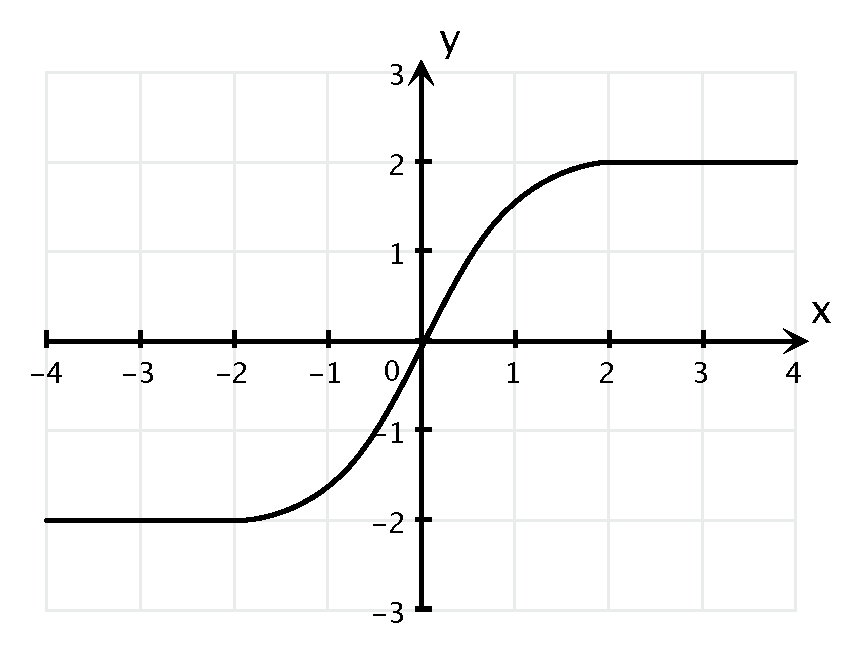
\includegraphics{graph_c.eps}}
\end{center}


\subsubsection{微分の基本公式}

\nquestion
導関数の定義式に基づいて次式を証明せよ。
\begin{enumerate}
\item $(f(x)\pm g(x))'=f'\pm g'$
\item $(kf(x))'=kf'$\quad($k$:定数)
\item $(f(x)g(x))'=f'g+fg'$
\item $\displaystyle\left(\frac{f(x)}{g(x)}\right)'=\frac{f'g-fg'}{g^2}$
  % \item $\displaystyle\{f(g(x))\}'=\frac{df}{dg}\frac{dg}{dx}$
\end{enumerate}

\nquestion
以下を導関数の定義に従って証明せよ。
\begin{enumerate}
\item $(2)'=0$
\item $(x^2)'=2x$
\item $(x^{-2})'=-2x^{-3}$
\item $(x^n)'=nx^{n-1}$ ($n$:正の整数)
\item $(x^n)'=nx^{n-1}$ ($n$:負の整数)
\item $(\sin x)'=\cos x$
\item $(\cos x)'=-\sin x$
\item $\displaystyle (\ln x)'=\frac{1}{x}$
\end{enumerate}

\nquestion
以下の導関数を求めよ。ここまでに証明した公式は用いてよい
\answer{
  (a) $y'=\frac{1}{\cos^2x}$\;
  (b) $y'=\sin x+x\cos x$\;
  (c) $y'=\frac{10}{(x-5)^2}$…分子が$x$を含まない形にまず変形してから微
  分すると楽\;
  (d) $y'=-\frac{1}{x^2}+\frac{1}{(x+1)^2}$…部分分数分解してから微分す
  るとよい}。
\begin{enumerate}
\item $y=\tan x$
\item $y=\log_a x$
\item $y=x\sin x$
% \item $\displaystyle y=\frac{5+x}{5-x}$
\item $\displaystyle y=\frac{1}{x(x+1)}$
\end{enumerate}

\subsection{複雑な関数の導関数}

\subsubsection{Chain Rule}
複雑な関数の導関数を求めるときには\bfindex{chain rule}を用いるとよい。
例えば,$y=(1+\sin 2x)^3$の導関数は以下のように求める。
\begin{align}
  y&=z^3\notag\\
  z&=1+w\notag\\
  w&=\sin u\notag\\
  u&=2x\notag
\end{align}
とおくと,
\begin{align}
  \frac{dy}{dx}
  =&\frac{dy}{dz}\cdot\frac{dz}{dw}\cdot\frac{dw}{du}\cdot\frac{du}{dx}\notag\\
  =&3z^2\cdot 1 \cdot \cos u\cdot 2\notag\\
  =&6(1+\sin 2x)^2\cdot \cos 2x \notag
\end{align}

\exercise
Chain ruleを用いて以下の導関数を求めよ
\answer{
(\ref{ditem:x^1.2}) $y'=1.2x^{0.2}$\;
(\ref{ditem:x^a}) $y'=ax^{a-1}$\;
(\ref{ditem:3x2-x-1}) $y'=4(6x-1)(3x^2-x-1)^3$\;
(\ref{ditem:tan(x2+2)}) $y'=\frac{2x}{\cos^2(x^2+2)}$\;
(\ref{ditem:logcos2x}) $y'=-2\tan x$\;
(\ref{ditem:log|x|}) $y'=\frac{1}{x}$\;
(\ref{ditem:loglogx}) $y'=\frac{1}{x\log x}$\;
(\ref{ditem:1/sqrt(x2+1)}) $y'=-\frac{x}{(x^2+1)\sqrt{x^2+1}}$\;
(\ref{ditem:sin10x2}) $y'=20x\cos x^2\cdot\sin^9x^2$\;
(\ref{ditem:xtan(x2)}) $y'=\tan x^2+\frac{2x^2}{\cos^2x^2}$\;
% (\ref{ditem:xe-x2}) $y'=(1-2x^2)e^{-x^2}$\;
% (\ref{ditem:log(x+sqrt(x2+1))}) $y'=\frac{1}{\sqrt{x^2+1}}$
}。
\textbf{これ以上変数を分解できないところまで分解すること。}

\begin{enumerate}
  \item \label{ditem:x^1.2}$y=x^{1.2}$ ($x>0$)
  \item \label{ditem:x^a}$y=x^a$ ($x>0$, $a$: 実数)
% \quad… 
%     $a$が整数の場合は前問で扱っている。
%     より一般的に$a$が実数の時には両辺の対数をとってから$x$で微分する。
  \item \label{ditem:3x2-x-1}$y=(3x^2-x-1)^4$…展開して計算しないこと
  \item \label{ditem:tan(x2+2)}$y=\tan(x^2+2)$
  \item \label{ditem:logcos2x}$y=\log\cos^2x$
  \item \label{ditem:log|x|}$y=\log|x|$, $(x<0)$
  \item \label{ditem:loglogx}$y=\log\log x$
  \item \label{ditem:1/sqrt(x2+1)}$\displaystyle y=\frac{1}{\sqrt{x^2+1}}$
  \item \label{ditem:sin10x2}$y=\sin^{10}x^2$
  \item \label{ditem:xtan(x2)}$y=x\tan x^2$\quad
    ($y=xz$, $z=\tan u$, $\cdots$ とおく)
%   \item \label{ditem:xe-x2}$y=xe^{-x^2}$ ($y=xz$, $z=e^{w}$, $\cdots$ とおく。)
%   \item \label{ditem:log(x+sqrt(x2+1))}$y=\log(x+\sqrt{x^2+1})$
\end{enumerate}

\subsubsection{逆関数・指数関数の微分}
逆関数や指数関数の導関数を求めるには,
式を微分しやすい形に変形した後,両辺を$x$で微分する。

\nquestion
以下の各関数の導関数を求めよ
\answer{
  (\ref{ditem:sin-1x}) $y'=\frac{1}{\sqrt{1-x^2}}$,~
  (\ref{ditem:cos-1x}) $y'=-\frac{1}{\sqrt{1-x^2}}$,~
  (\ref{ditem:tan-1x}) $y'=\frac{1}{1+x^2}$, ~
  (\ref{ditem:ex}) $y'=e^x$,~
  (\ref{ditem:ax}) $y'=a^x\log a$,~
  (\ref{ditem:xx}) $y'=x^x(\log x+1)$。
}。
ただし,ここまでの問題で証明していない公式を使わないこと。
どうしても使いたいときには必ず証明をすること。
\begin{enumerate}
\item \label{ditem:sin-1x}$\displaystyle y=\sin^{-1}x,\quad(-\pi/2\le y\le\pi/2)$
\item \label{ditem:cos-1x}$\displaystyle y=\cos^{-1}x,\quad(0\le y\le\pi)$
\item \label{ditem:tan-1x}$\displaystyle y=\tan^{-1}x,\quad(-\pi/2< y<\pi/2)$
\item \label{ditem:ex}$y=e^x$
\item \label{ditem:ax}$y=a^x$ $(a>0)$
\item \label{ditem:xx}$y=x^x$ $(x>0)$
\end{enumerate}
% \nquestion
% 前問で計算したように$\sin^{-1}x$と$\cos^{-1}x$の導関数は互いに符号が異
% なるだけである。その理由を説明せよ。

% \subsection{微分と図形}
% \nquestion
% \begin{enumerate}
% \item $x=2t+1$のグラフを書きなさい。
% \item $x=2t+1$の傾きが$t$の値とともにどう変わるかを,先に書いたグラフ
%   を見て書きなさい。
% \item 前問の結果をもとに $x=2t+1$の微分値がどのような値になるかを説明
%   しなさい。
% \end{enumerate}

\subsection{微分と定性的表現}

\nquestion
以下の定性的表現を数式で表しなさい。
ただし,ある量の変化とは,
\begin{quote}
  \textbf{変化=「後の量」ー「始めの量」}
\end{quote}
で与えられることに注意しなさい
\answer{
% (\ref{ditem:weight})~
(\ref{ditem:displaycement})~$\Delta x =x(t_2)-x(t_1)$~
(\ref{ditem:avrvel}) $\displaystyle \frac{\Delta x}{\Delta t}=\frac{x(t_2)-x(t_1)}{t_2-t_1}$\\
(\ref{ditem:dV>0}) 物体の体積を$V$とする。$\dot{V}<0$\\
(\ref{ditem:v=0}) $\dot{x}(0)=0$ ($x$は物体の位置)\\
(\ref{ditem:dT=0}) $\dot{T}=0$ ($T$は物体の温度)\\
(\ref{ditem:dT(t0)=0}) $\dot T(t_0)=0$ ($T$は物体の温度)\\
(\ref{ditem:dT}) $\dot{T}=k(T_0-T)$ ($k$は正の定数)
}
。

\begin{enumerate}
% \item\label{ditem:weight} ある月の体重は前の月の体重から1割減った。
\item\label{ditem:displaycement} 時刻$t_1$から時刻$t_2$までの間の位置$x(t)$
  の変化を変位$\Delta x$とよぶ。
\item\label{ditem:avrvel} 時刻$t_1$から時刻$t_2$までの間の位置$x$
  の平均変化率を$\displaystyle\frac{\Delta x}{\Delta t}$で表す。
\item\label{ditem:dV>0} ある物体の体積が時間とともに減少している。
\item\label{ditem:v=0} ある物体が時刻$t=0$において静止している。
\item\label{ditem:dT=0} ある物体の温度は時間によらず一定である。
\item\label{ditem:dT(t0)=0}
  ある物体の温度が時刻$t_0$に極小値もしくは極大値になる。
\item\label{ditem:dT} ある物体が一定の温度$T_0$の恒温槽にあるとする。このとき物体の温度$T$は$T_0$に近づいていくが、その時間変化率は温度差に比例する。
\end{enumerate}


%%%%%%
\nquestion 以下の問いに答えなさい。
\begin{enumerate}
\item 以下の定性的表現を数式で表しなさい\answer{
(\ref{ditem:usa-C}) ある年(第$t$年)のうさぎの個体数を$n_t$とおく。
$n_t=n_{t-1}$
(\ref{ditem:usa+10}) $n_t=1.1n_{t-1}$ ($n_t$は問(\ref{ditem:usa-C})と同様)\\
% (\ref{ditem:usa-10}) $n_t=0.9n_t$ ($n_t$は問(\ref{ditem:usa-C})と同様)\\
(\ref{ditem:usa-cresc}) 以下ではうさぎの個体数を$n_r(t)$とおく。
$\dot{n}_r=C$ ($C$は定数)
(\ref{ditem:usa-moltocresc}) $\dot{n}_r=kn_r$ ($k$は定数)\\
(\ref{ditem:Pusa-okami})
以下の問では狼の個体数を$n_w(t)$, うさぎと狼の遭遇確率を$P$とおく。
$P=kn_rn_w$ ($k$は正の定数)\\
(\ref{ditem:usa-change})(\ref{ditem:wolf-change})
\begin{align*}
	\begin{cases}
	\dot{n}_r&=an_r-bP\\
		&=an_r-bkn_rn_w\quad (a,bは正の定数)\\
	\dot{n}_w&=-cn_w+dP\\
		&=-cn_w+dkn_rn_w\quad (c,d は正の定数)
	\end{cases}
\end{align*}
}。
\begin{enumerate}
	\item\label{ditem:usa-C} ある島に住むうさぎのある年の個体数と前年の個体数は常に同じである。
	\item\label{ditem:usa+10} ある島に住むうさぎのある年の個体数は前年の個体数より常に1割多い。
% \item\label{ditem:usa-10} ある島に住むうさぎのある年の個体数は前年の個体数より常に1割少ない。
	\item\label{ditem:usa-cresc}
	ある島のうさぎは増加しており,その増加率は一定である。
  (以下ではうさぎの個体数を実数として扱う)
	\item\label{ditem:usa-moltocresc}
  ある島に住むうさぎは増加しており,その増加率は個体数に比例する。
	\item\label{ditem:Pusa-okami}
  ある島にはうさぎと狼が住んでいる。うさぎと狼の遭遇確率は,うさぎと狼
  の個体数の積に比例する。
	\item\label{ditem:usa-change}
  ある島のうさぎの増加率は,個体数に比例する増加率と, うさぎと狼の
  遭遇確率に比例する減少率の和によって表される。
  ただし,狼がいなければうさぎは常に増加する。
	\item\label{ditem:wolf-change}
  ある島の狼の増加率は,個体数に比例する減少率と, うさぎと狼の
  遭遇確率に比例する増加率の和によって表される。
  ただし,狼は餌になるうさぎがいなかったら減少する。
\end{enumerate}
\item 前問の(\ref{ditem:usa-change})と(\ref{ditem:wolf-change})で定式化した微分方程式は,捕食者と被食者の個体変動モデルとして有名であり,Lotka-Volterra方程式とよばれている。
  実際にこの方程式で予測されるような個体数の変動は自然界でしばしば観察されることが報告されている。
  さて,うさぎと狼の個体数が一定となる条件を,Lotka-Volterra方程式より求めなさい。
\end{enumerate}

%%%%%%
\nquestion
水槽の底にある管からポンプで水を入れたところ、
単位時間あたりに水槽に入る水の量は水槽内の水の量に反比例して
いた。
また, この水槽の底には小さな穴があいており、単位時間あたり一定の量の水
が漏れていた。
\begin{enumerate}
\item 必要な変数を定義し、水槽の中の水の量の時間変化率を表す方程式を
  書きなさい
\answer{
水槽中の水の量を$V$, 単位時間あたりに水槽から漏れる水の量を$a$とおく。
題意より次式が成り立つ。
  \begin{align}
    \displaystyle \dot{V}=\frac{k}{V}-a\notag
  \end{align}
  ここで、$k$は正の定数である。}。
\item しばらく水を入れ続けているとやがて水槽の水の量が変化しなくなっ
  た。このときの水の量を求めなさい
\answer{$\displaystyle V=\frac{k}{a}$}。
\end{enumerate}


\subsection{微分と接線}

\nquestion
以下の問に答えなさい。
\begin{enumerate}
\item $y=2x^2$の$x=1$における\bfindex[せっせん]{接線}(\nmindex{tangent line})
を表す方程式は?
\answer{
$y-2=4(x-1)$
}
\item 原点を中心とする半径1の円のうち$y>0$の部分の、$x=\frac{1}{2}$に
  おける接線は?
\answer{
% $\frac{dy}{dx}=-\frac{x}{y}=-\frac{x}{\sqrt{1-x^2}}$より,
% $x=\frac{1}{2})$における接線の傾きは...
$y-\frac{\sqrt{3}}{2}=-\frac{1}{\sqrt{3}}(x-\frac{1}{2})$
\;(ヒント:\;$x^2+y^2=1$の両辺を$x$で微分すれば$y'$を簡単に計算できる)
}
\item $xy$平面における以下の曲線の$t=1$における接線は?
\answer{
$y-1=2x$\;
(ヒント:\;$\displaystyle\frac{dy}{dx}=\frac{dy}{dt}\frac{dt}{dx}$を使うと便利)
}
\begin{align}
  \begin{cases}
      x=t-1 \\
      y=t^2
    \end{cases}\quad\mbox{($t$は実数)}\notag
\end{align}
\item  $xy$平面における以下の曲線の$t=1$における接線は?
  \answer{
    $y=\frac{1}{2}(x-1)$
  }
  \begin{align}
    \begin{cases}
      x=t^2 \\
      y=t-1
    \end{cases}\quad\mbox{($t$は正の実数)}\notag
  \end{align}
\end{enumerate}

\nquestion 以下の問に答えなさい。
\begin{enumerate}
\item
2曲線$y=f(x)$と$y=g(x)$が点$(x_0,y_0)$で接する条件を述べなさい
\answer{
$y_0=f(x_0)=g(x_0)$,
$f'(x_0)=g'(x_0)$
}
。
\item $f(x)$と$g(x)$を$x$の多項式であるとして,以下の問に答えなさい。
  \begin{enumerate}
  \item
    方程式$f(x)=g(x)$が重根をもつならば,
    2曲線$y=f(x)$と$y=g(x)$は接点をもつことを示しなさい
    \answer{
    方程式$f(x)=g(x)$が重根をもつならば
    次式を満たす$x_0$および多項式$h(x)$が存在する。
    \begin{align}
%       \label{eq:contact-condition}
      f(x)-g(x)=(x-x_0)^2h(x)\notag
    \end{align}
    このとき,$x=x_0$で前問で述べた条件($f(x_0)=g(x_0)$, $f'(x_0)=g'(x_0)$)が
    成り立つことを示せば良い。
    }。
  \item
     前問の逆も成り立つことを証明しなさい。すなわち
    2曲線$y=f(x)$と$y=g(x)$が接点をもつならば,
    方程式$f(x)=g(x)$が重根をもつことを示しなさい
    \answer{
      接点の$x$座標を$x=x_0$とすると,以下が成立する。
      \begin{align}
        \label{eq:contact-cond1}
        f(x_0)&=g(x_0)\\
        \label{eq:contact-cond2}
        f'(x_0)&=g'(x_0)
      \end{align}
      式(\ref{eq:contact-cond1})より,$x=x_0$は$f(x)-g(x)=0$の解なので,
      以下を満たす多項式$k(x)$が存在する。
      \begin{align}
        \label{eq:contact-cond3}
        f(x)-g(x)=(x-x_0)k(x)
      \end{align}
      上式を微分すると
      \begin{align}
        f'(x)-g'(x)=k(x)+(x-x_0)k'(x)
      \end{align}
      上式が式(\ref{eq:contact-cond2})を満たす条件は,$k(x)=(x-x_0)h(x)$,
      ($h(x)$は多項式)が成り立つことである。従って式
      (\ref{eq:contact-cond2})は以下のように書き直せる。
      \begin{align}
        f(x)-g(x)=(x-x_0)^2h(x)
      \end{align}
      すなわち,方程式$f(x)-g(x)=0$は重根をもつことがわかる。
    }。
  \end{enumerate}
\end{enumerate}
\comment
以上より,2つの多項式$f(x)$と$g(x)$が接点をもつ条件は,$f(x)=g(x)$が
重根をもつことであることがわかる。

\subsection{高次導関数}

\nquestion
以下の$n$次導関数を求めよ
\answer{
(\ref{Ditem:e^x}) $f^{(n)}(x)=e^x$\\
(\ref{Ditem:sinx}) $f^{(n)}(x)=
\begin{cases}
  (-)^m\cos x & (n=2m+1)\\
  (-)^m\sin x & (n=2m)
\end{cases}$ ($m=0,1,2,.\ldots$)\\
(\ref{Ditem:cosx})
 $f^{(n)}(x)=
\begin{cases}
  (-)^{m+1}\sin x & (n=2m+1)\\
  (-)^m\cos x & (n=2m)\quad(m=0,1,2,.\ldots)
\end{cases}$
}。
\begin{enumerate}
\item\label{Ditem:e^x} $f(x)=e^x$
\item\label{Ditem:sinx} $f(x)=\sin x$
\item\label{Ditem:cosx} $f(x)=\cos x$
\end{enumerate}
\nquestion
以下の関数をそれぞれ4階微分まで求め,それに基づいて,$n$階微分
$f^{(n)}$を推測せよ
\answer{
(\ref{eq:fnOFx^k}) $
f^{(n)}(x)=
\begin{cases}
\displaystyle
\frac{k!}{(k-n)!}x^{k-n}&(n\le k)\\
0 & (n>k)
\end{cases}$\\
(\ref{eq:fvOFlog(1+x)})
$\displaystyle f^{(n)}(x)=
\begin{cases}
  \log(1+x) & (n=0)\\
\displaystyle (-)^{n-1}\frac{(n-1)!}{(1+x)^{n}}& (n>0)
\end{cases}$
}。
その推測が正しいことを数学的帰納法で証明せよ。
\begin{enumerate}
\item\label{eq:fnOFx^k} $f(x)=x^k$ ($k$: 正の整数)
\item\label{eq:fvOFlog(1+x)} $f(x)=\log (1+x)$
% \item $\displaystyle f(x)=\frac{1}{1-x}$
\end{enumerate}
\nquestion
$x=A\sin(\omega t+\phi)$が次式を満たすような$\omega$の値を求め
なさい。ただし, $A$, $\phi$は定数である。
\begin{align}
  \ddot{x}=-kx\notag
\end{align}

\subsection{マクローリン展開とテイラー展開}

\subsubsection{マクローリン展開}

様々な関数の振舞を解析する際,三角関数等のように値を簡単に求めることが
できない謎の関数が含まれていると大変困る。
そこで,例えば謎の関数$f(x)$の$x=0$の近傍での値や振舞いを知りたい場合
には,次式のように$f(x)$を$x$の級数で表現できれば解析が容易になる。
\begin{align}
  f(x)=\sum_{n=0}^{\infty}a_nx^n\notag
\end{align}

\nquestion
$a_n$を求める方法を考えてみよう。
よい近似式を得るには$x=0$における両者の$n$次微分係数($n=0,...,\infty)$
が全て等しくなるように係数$a_n$を決める必要がある。

関数$y=f(x)$が$x=0$を含むある区間で$C^\infty$級
\footnote{関数$f(x)$が区間$I$で$n$回微分可能であり,$f^{(n)}(x)$が
  区間$I$で連続なとき,関数$f(x)$は区間$I$で$C^n$級であるという。}の場
合について係数$a_n$を決定し,$f(x)$を無限級数で表すと以下のよう
になることを証明しなさい。
\begin{align}
  f(x)=\sum_{n=0}^{\infty}\frac{f^{(n)}(0)}{n!}x^n
 \label{eq:Maclaurin}
\end{align}

\comment
ある関数$f(x)$を上記のように級数展開することを
\bfindex[まくろーりんてんかい]{マクローリン展開}
(\nmindex{Maclaurin expansion})
\footnote{
%スコットランドの数学者\href{https://ja.wikipedia.org/wiki/コリン・マクローリン}{コリン・マクローリン}\index{マクローリン}(Colin Maclaurin\index{Maclaurin, Colin}, 1698-1746)にちなむ。
マクローリンは11歳でグラスゴー大学に入学, 19歳にはアバディーン大学の教授,その後
ニュートンに才能を認められ,ニュートンによる推薦状によって27歳でエジンバラ大学の教授に就任している。
マクローリンは最も若く教授になった人物として約300年にわたって記録保持者だったが
2008年にこの記録はアメリカ人の\href{https://en.wikipedia.org/wiki/Alia_Sabur}{Alia Sabur}が18歳で韓国の大学教授に就任することで破られる。
マクローリン自身はテイラー展開(後述)を数学的な議論に用いたが,その業績を評価され,
テイラー展開を$x=0$において用いた場合はマクローリン展開と呼ばれるようになった。
マクローリンはニュートンの業績についても書籍にまとめている
(\href{https://archive.org/details/anaccountsirisa00murdgoog}{"An Account of Sir Issac Newton's Philosophical Discoveries", 1775})。
}という。

\nquestion
以下の問いに答えなさい
\answer{
(\ref{itemM:(1+x)^n}) $\displaystyle(1+x)^n=\sum_{m=0}^n\frac{n!}{m!(n-m)!}x^m$
(\ref{itemM:Me^x}) $\displaystyle e^x=\sum_{n=0}^\infty\frac{x^n}{n!}$~
(\ref{itemM:sinx}) $\displaystyle \sin x=\sum_{m=0}^\infty\frac{(-)^{m}}{(2m+1)!}x^{2m+1}$~
(\ref{itemM:cosx}) $\displaystyle \cos x=\sum_{m=0}^\infty\frac{(-)^m}{(2m)!}x^{2m}$~
}。
\begin{enumerate}
\item\label{itemM:(1+x)^n} $(1+x)^n$ をマクローリン展開しなさい。
その結果より,$x\ll 1$のとき次式が成り立つことを示しなさい。
\begin{align}
  (1+x)^n\simeq 1+nx\notag
\end{align}
実際に $1.1^2$, $1.1^3$...等でこの近似がどの程度正しいか確認しなさい。
\item\label{itemM:Me^x} $e^x$ をマクローリン展開しなさい。
\item\label{itemM:sinx} $\sin x$ をマクローリン展開しなさい。
  また,$x\ll 1$のとき次式が成り立つことを示しなさい。
  \begin{align}
    \sin x\simeq x\notag
  \end{align}
\item\label{itemM:cosx} $\cos x$ をマクローリン展開しなさい。
  また,$x\ll 1$のとき次式が成り立つことを示せしなさい。
  \begin{align}
    \cos x\simeq 1-\frac{1}{2}x^2\notag
  \end{align}
\item $x=0$, $x=\frac{\pi}{6}$の場合それぞれについて,$\sin x$, $\cos x$の真値と上記による近似値がどの程度異なるか計算しなさい。
%\item $\sin 1.8^{\circ}$, $\cos 1.8^{\circ}$をそれぞれ手計算で見積もり,
%  正確な値($\sin 1.8^{\circ}=0.031411\cdots$, $\cos 1.8^{\circ}=0.999507\cdots$)との差がどの程度かを確認せよ。
\item $\displaystyle \lim_{x\to 0}\frac{\sin x}{x}=1$
  をマクローリン展開を用いて証明しなさい。
\item $e$の値を求める多項式をつくりなさい。
\end{enumerate}

\exercise
$\displaystyle f(x)=\frac{1}{1-x}$\quad$(|x|<1)$をマクローリン展開により無限級数に展開しなさい
\answer{$\displaystyle\frac{1}{1-x}=\sum_{n=0}^\infty x^n$}。


\subsubsection{テイラー展開}

マクローリン展開は,関数$f(x)$を$x=0$のまわりで級数展開するものであった。
同様にして,関数$f(x)$を$x=a$のまわりで無限級数に展開,すなわち,
\begin{align*}
	f(x)=\sum_{n=0}^{\infty}a_n(x-a)^n
\end{align*}
と展開する方法を
\bfindex[ていらーてんかい]{テイラー展開}
\footnote{
テイラー展開はスコットランドの数学者・天文学者のジェームス・\nmindex{グレゴリー}
(James Gregory\index{Gregory, James}, 1638-1675, スコットランド)による発案。
イギリスの数学者ブルック・\nmindex{テイラー}
(Brook Taylor\index{Taylor, Brook}, 1685-1731)が1715年に出版した著書にこの
級数展開法を記したのが後にラグランジュの目に止まり,注目されるようになった。
%https://en.wikipedia.org/wiki/Brook_Taylor
}
(\nmindex{Taylor expansion})
とよぶ。
展開式は 次式の通り。
\begin{align}
  f(x)=\sum_{n=0}^{\infty}\frac{f^{(n)}(a)}{n!}(x-a)^n
  \label{eq:Taylor}
\end{align}
関数$f(x)$の$x=0$におけるテイラー展開がマクローリン展開に一致する。

\nquestion
テイラー展開を与える式(\ref{eq:Taylor})を,マクローリン展開の場合と同様に導きなさい。

\exercise
以下の関数をテイラー展開しなさい。
\begin{enumerate}
\item $f(x)=\sin x$\quad($x=\pi$のまわりで)
\item $f(x)=\log x$\quad($x=1$のまわりで)
\end{enumerate}

\subsection{オイラーの公式}

\subsubsection{オイラーの公式の導出}
\nquestion 以下の問いに答えなさい。
\begin{enumerate}
\item マクローリン展開を用いてオイラー
\footnote{レオンハルト・\nmindex{オイラー}(
Leonhard Euler\index{Euler, Leonhard},
1707年4月15日 - 1783年9月18日)はスイス生まれの数学者,物理学者であり、天文学者。
整数論,解析学,複素数論,物理学等に多くの業績を残し,人類史上最も多くの論文を書いた数学者と言われている。
流体力学や剛体の力学の基礎を築いたのもオイラー。
% https://ja.wikipedia.org/wiki/%E3%83%AC%E3%82%AA%E3%83%B3%E3%83%8F%E3%83%AB%E3%83%88%E3%83%BB%E3%82%AA%E3%82%A4%E3%83%A9%E3%83%BC
}
の公式\index{おいらーのこうしき@オイラーの公式}と呼ばれる次式を証明しなさい。
  \begin{align}
    e^{ix}=\cos x + i \sin x \notag
  \end{align}
\item $e^{ix}$の大きさを求めなさい。
\item 「\nmindex[おいらーのほうせき]{オイラーの宝石}」と呼ばれる次式を証明しなさい。
  \begin{align}
    e^{i\pi}=-1 \notag
  \end{align}
\item $i^i$が実数であることを示しなさい。
\item 「\nmindex[ど・もあぶるのこうしき]{ド・モアブルの公式}」
と呼ばれる次式を証明しなさい。
  \begin{align}
    (\cos\theta+i\sin\theta)^n=\cos n\theta+i\sin n\theta\notag
  \end{align}
\end{enumerate}

\subsubsection{オイラーの公式と三角関数の公式}

\nquestion 以下の問いに答えなさい。
\begin{enumerate}
\item
オイラーの公式を用いて以下を証明しなさい。
\begin{enumerate}
\item $\sin(x\pm y)=\sin x\cos y\pm\sin y\cos x$
\item $\cos(x\pm y)=\cos x\cos y\mp\sin y\sin x$
\item $\displaystyle\sin 2x=2\sin x\cos x$
\item $\displaystyle\cos 2x=\cos^2x-\sin^2x$
\end{enumerate}
\item 前問の結果をもとに以下を導きなさい。
\begin{enumerate}
\item $\displaystyle\sin x+\sin y=2\sin(\frac{x+y}{2})\cos(\frac{x-y}{2})$
\item $\displaystyle\cos x+\cos y=2\cos(\frac{x+y}{2})\cos(\frac{x-y}{2})$
\end{enumerate}
% \item 前問の(a)と(b)をド・モアブルの公式を用いて導きなさい。
% \item オイラーの公式の両辺を微分すると
%   \begin{align}
%     ie^{ix}=\frac{d}{dx}\cos x + i\frac{d}{dx}\sin x
%   \end{align}
%   となる。左辺にオイラーの公式を代入すると次式が得られる。
%   \begin{align}
%     ie^{ix}=i(\cos x + i\sin x)=-\sin x + i\cos x
%   \end{align}
%   以上の2式の実部と虚部をそれぞれ比べると、$\sin x$, $\cos x$の
%   微分が得られることがわかる。同様にして$\sin x$, $\cos x$の
%   $n$階微分を求めなさい。
\item 以下の式で$a$, $b$が与えられたとき,どのように$r$, $\phi$を
  決めたら等式が成り立つか?
  \begin{align}
    a\sin x+b\cos x=r\sin(x+\phi)\notag
  \end{align}
ヒント)左辺を$r(\cos\phi\sin x+\sin\phi\cos x)$の形に変形する。
\item 以下を$r\sin(x+\phi)$の形に変形せよ
\answer{
%    (\ref{item:sinx+cosx}) $\sqrt{2}\sin(x+\frac{\pi}{4})$
   (\ref{item:sqrt(3)sinx+cosx}) $2\sin(x+\frac{\pi}{6})$
   (\ref{item:sinx-sqrt(3)cosx}) $2\sin(x-\frac{\pi}{3})$
}。
  \begin{enumerate}
%    \item\label{item:sinx+cosx} $\sin x+\cos x$
   \item\label{item:sqrt(3)sinx+cosx} $\sqrt{3}\sin x+\cos x$
   \item\label{item:sinx-sqrt(3)cosx} $\sin x-\sqrt{3}\cos x$
  \end{enumerate}
\end{enumerate}

\subsubsection{オイラーの公式と複素数\label{sec:Euler-complex}}

複素数$z=a+bi$は偏角$\theta=\arg z$を用いて次のように
書くことができる。
\begin{align*}
%   \label{eq:complex}
  z&=|z|e^{i\theta}\\
  &=|z|(\cos\theta+i\sin\theta)
\end{align*}

\nquestion 以下の問いに答えなさい。
\begin{enumerate}
\item $|z|$, $\cos\theta$,$\sin\theta$を$a$, $b$で表しな
  さい。
\item 虚数単位$i$を$re^{i\theta}$の形に表しなさい。
\item 複素数$z$に虚数単位$i$をかける演算は,複素空間上で原点周りに$\frac{i}{2}$回転する変換と等価であることを説明しなさい。
\item 複素数$z_1$, $z_2$の大きさおよび\nmindex[へんかく]{偏角}と,
  以下の各値の大きさおよび偏角はどのような関係にあるか。
  オイラーの公式を利用して答えなさい。
  \begin{enumerate}
  \item 複素数$z_1$と$z_2$の積$z_1z_2$
  \item 複素数$z_1$と$z_2$の商$z_1/z_2$
  \end{enumerate}
\item 以下の各複素数の大きさと偏角を求めなさい。
\index{ふくそすう@複素数!のおおきさ@---の大きさ}
\index{ふくそすう@複素数!のへんかく@---の偏角}
  また,各値を複素平面上に図示しなさい。
  ここで,偏角は$(-\pi,\pi]$の範囲で答えること。
  必要な演算には,前問の結果に基づいて幾何学的に解を考える方法と,
  オイラーの公式を利用して計算する方法の2通りで行い、両者で結果が等しくな
  ることを確認しなさい
  \answer{以下は各値$z$に対する$(|z|,\arg z)$を表す。\\
(\ref{eitem:z1}) $\displaystyle(1,-\frac{\pi}{2})$~
(\ref{eitem:z2}) $\displaystyle(\sqrt{2}, \frac{\pi}{4})$~
% (\ref{eitem:z3}) $\displaystyle(2,\frac{2}{3}\pi)$~
(\ref{eitem:1/z_1}) $\displaystyle(1, \frac{\pi}{2})$~\\
(\ref{eitem:1/z_2}) $\displaystyle(\frac{1}{\sqrt{2}},-\frac{\pi}{4})$~
(\ref{eitem:z_1^4}) $(1,0)$~
(\ref{eitem:z_2^4}) $(4,\pi)$~
% (\ref{eitem:z_3^3}) $(8,0)$\\
(\ref{eitem:z_2barz_2}) $(2,0)$~
% (\ref{eitem:z_2/barz_2}) $\displaystyle(1,\frac{\pi}{2})$~
% (\ref{eitem:z_3/z_1}) $\displaystyle(2,-\frac{5}{6}\pi)$~
% (\ref{eitem:z_1z_3/z_2}) $\displaystyle(2, -\frac{\pi}{6})$
}。
  \begin{enumerate}
  \item\label{eitem:z1} $z_1=-i$
  \item\label{eitem:z2} $z_2=(1+i)$
%   \item\label{eitem:z3} $\displaystyle z_3=-1+\sqrt{3}i$
  \item\label{eitem:1/z_1} $\displaystyle\frac{1}{z_1}$
  \item\label{eitem:1/z_2} $\displaystyle\frac{1}{z_2}$
  \item\label{eitem:z_1^4} $z_1^4$
  \item\label{eitem:z_2^4} $z_2^4$
%   \item\label{eitem:z_3^3} $z_3^3$
  \item\label{eitem:z_2barz_2} $z_2\bar{z}_2$
%   \item\label{eitem:z_2/barz_2} $\displaystyle\frac{z_2}{\bar{z}_2}$
%   \item\label{eitem:z_3/z_1} $\displaystyle\frac{z_3}{{z}_1}$
%   \item\label{eitem:z_1z_3/z_2} $\displaystyle\left(\frac{z_1z_3}{z_2}\right)^2$
  \end{enumerate}
\item 次式が1の$n$乗根であることを示しなさい。
  \begin{align}
    z=\cos\frac{2\pi}{n}+i\sin\frac{2\pi}{n}\notag
  \end{align}
\end{enumerate}

%%%%%%
\nquestion
複素空間上の点$w$を$z$の周りに反時計回りに$\frac{\pi}{2}$回転した時,
どのような点$w_z$に写像されるかを考えたい。
以下の問に答えなさい
\answer{
(1) $w_z=1+2i$~
(2)(a) $w'=1$~
(b) $w''=i$~
(d) $w'=w-z$~
(e) $w_z=(w-z)i+z$~
}。
\begin{enumerate}
\item $z=1+i$, $w=2+i$の場合について,幾何学的に考えることで,点$w_z$を表す複素数を答えなさ
  い。
\item
  座標軸を平行移動して$z$が原点になるように取り直す。
  もとの座標系を$L_1$, 新しい座標系を$L_2$とする。
  \begin{enumerate}
    \item $L_1$座標系における点$w=2+i$は,$L_2$座標系ではどのような複素数$w'$で表されるか。
    \item $w'$を$L_2$座標系の原点周りで$\frac{\pi}{2}$回転した点を表す複素数
  $w''$を$L_2$座標系で答えなさい。
    \item $w''$を$L_1$座標系での複素数で表すと (1)の結果と同じになる
  ことを確認しなさい。
    \item 任意の点$w$を題意の写像により$w_z$に写す場合について考える。$w_z$を表す$L_2$上の複素数$w'$を$w$, $z$を用いて答えなさい。
  \item $L_1$座標系における点$w_z$を表す複素数を$w$, $z$を用いて答えなさい。
\end{enumerate}
\end{enumerate}


\newpage

\section{積分}

\subsection{不定積分}

\subsubsection{不定積分の定義}
\textbf{微分の逆演算}を\bfindex[ふていせきぶん]{不定積分}
(\nmindex{indefinite integral})とよぶ。
すなわち,ある関数$f(x)$に対して、導関数が$f(x)$となる関数の集合を求め
る演算が不定積分である。

$F'(x)=f(x)$のとき,
\begin{align}
  \int f(x)dx=F(x)+C\notag
\end{align}
と書いて左辺を関数$f(x)$の\textbf{不定積分},
$f(x)$を\textbf{被積分関数},
定数$C$を\bfindex[せきぶんていすう]{積分定数}(\nmindex{constant of integration}),
$F(x)$を$f(x)$の\bfindex[げんしかんすう]{原始関数}(\nmindex{antiderivative})とよぶ。
上式の左辺は次のように書くこともある。
\begin{align}
  \int dx f(x)\notag
\end{align}


\subsubsection{不定積分の幾何学的意味}
\nquestion
以下の数式の幾何学的意味を説明しなさい。
\begin{enumerate}
\item $\displaystyle\int 0 dt=C$\quad ($a$は定数,$C$は積分定数)
\item $\displaystyle\int a dt=at+C$\quad ($a$は定数,$C$は積分定数)
\end{enumerate}


\subsubsection{不定積分の公式\label{sec:integration-formula}}

導関数は定義式にしたがって計算すれば、原理的には求めることが出来る。
しかし、不定積分は「微分すれば$\int$の中身(被積分関数)になるものはな
にか」と問うクイズのようなものであり,残念ながら微分のように決まった解
き方は無い。
\textbf{変数置換,部分分数分解,部分積分}などにより,
\textbf{少しでも積分しやすそうな形に変形}を試みながら,
被積分関数が何かの微分になってないかを考えることが解法である。
このため,少なくとも以下の微分公式程度は覚えておく必要がある。
\begin{enumerate}
\item $(x^a)'=ax^{a-1}$%, \quad$(a\ne 0)$
\item $(\sin x)'=\cos x$
\item $(\cos x)'=-\sin x$
\item $\displaystyle(\log |x|)'=\frac{1}{x}\quad (x\ne 0)$
\item $(e^x)'=e^x$
\end{enumerate}
%% \begin{align}
%%   (x^a)'&=nx^{a-1}, (a\in\Real)\notag\\
%%   (\sin x)'&=\cos x \notag\\
%%   (\cos x)'&=-\sin{x} \notag\\
%%   (\log x)'&=\frac{1}{x}\quad (x>0) \notag\\
%%   (e^x)'&=e^x \notag
%% \end{align}
\nquestion
例えば,上記(2)式の両辺を積分すると
\begin{align}
  \int(\sin x)'dx&=\int\cos x dx\notag\\
  \sin x + C&= \int\cos x dx\notag
\end{align}
すなわち,次のような積分公式を得ることができる。
\begin{align}
\int\cos x dx=\sin x +C\notag
\end{align}

上の微分公式から積分公式をそれぞれ導きなさい。

\exercise
以下の不定積分を求めなさい
\answer{以下で(他の問の答においても)$C$は積分定数。
% (\ref{item:int x^2})     $\displaystyle\frac{1}{3}x^3+C$
% (\ref{item:int x^(3/2)}) $\displaystyle\frac{2}{5}x^{5/2}+C$
% (\ref{item:int x})       $\displaystyle\frac{1}{2}x^2+C$
(\ref{item:int x^(1/2)}) $\displaystyle\frac{2}{3}x^{3/2}+C$
(\ref{item:int 1/x^(1/2)})$\displaystyle2\sqrt{x}+C$
(\ref{item:int 1/x})     $\displaystyle\log|x|+C$
(\ref{item:int 1/(1-x)})     $\displaystyle -\log|x-1|+C$
(\ref{item:int 1/x^(3/2)})$\displaystyle-\frac{2}{\sqrt{x}}+C$
(\ref{item:int 1/x^2})   $\displaystyle-\frac{1}{x}+C$
}。また,答えを微分することによって検算せよ。
\begin{enumerate}
% \item\label{item:int x^2} $\displaystyle \int x^2 dx$
% \item\label{item:int x^(3/2)} $\displaystyle \int x\sqrt{x} dx$
% \item\label{item:int x} $\displaystyle \int x dx$
\item\label{item:int x^(1/2)} $\displaystyle \int \sqrt{x} dx$
\item\label{item:int 1/x^(1/2)} $\displaystyle \int \frac{1}{\sqrt{x}} dx$
\item\label{item:int 1/x} $\displaystyle \int \frac{1}{x} dx$
\item\label{item:int 1/(1-x)} $\displaystyle \int \frac{1}{1-x} dx$
\item\label{item:int 1/x^(3/2)} $\displaystyle \int \frac{1}{x\sqrt{x}} dx$
\item\label{item:int 1/x^2} $\displaystyle \int \frac{1}{x^2} dx$
\end{enumerate}


\subsection{定積分}
\subsubsection{定積分の定義}
\begin{figure}[h]
  \begin{center}
    \resizebox{6cm}{!}{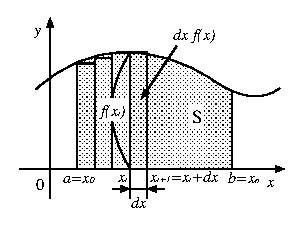
\includegraphics{SbySum.eps} }
    \caption{\label{fig:SbySum}
      面積と区分法}
  \end{center}
\end{figure}
\begin{figure}[h]
  \begin{center}
    \resizebox{6cm}{!}{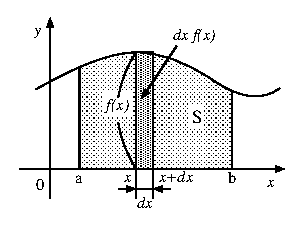
\includegraphics{integration.eps} }
    \caption{\label{fig:integration}
      定積分と面積}
  \end{center}
\end{figure}

% 水たまりの表面積を求めたい時には、どのようにしたら良いだろう。
% たとえば、正方形のタイルを水たまりと同じ形に敷き詰めて、
% タイル一枚の面積とその枚数を掛けあわせれば、おおよその面積は求めること
% が出来る。精度を高くしたければ、小さめのタイルを使えば良い。


ある関数$y=f(x)$と$x=a$, $x=b$,そして$x$軸で囲まれた面積$S$を
求める方法を考えてみよう。
例えば,この区間を$n$個の区間に分割し、それぞれを長方形とみなして計算
した面積の和$S_n$で近似的に計算することができる(図\ref{fig:SbySum})。
すなわち,
\begin{align}
  S_n&=f(x_0)\Delta x+f(x_1)\Delta x+\cdots+f(x_{n-1})\Delta x\notag\\
  &=\sum_{i=0}^{n-1}f(x_i)\Delta x
\end{align}
ただし,$a=x_0$, $b=x_n$であり,$\Delta x$は分割した1区間の幅
($\Delta x=x_{i+1}-x_i$)である。
この分割数を無限個にした極限では$S_n$は真の面積$S$に近付くと考えられる。
すなわち,
\begin{align}
  S=\lim_{n\to \infty}\sum_{i=0}^nf(x_i)\Delta x
\end{align}
ここで,$\displaystyle\lim_{n\to \infty}\sum_{i=0}^n$を$\displaystyle\int_a^b$,
微小幅である$\Delta x$を$dx$と簡単化のためおき直すと,面積は次式のように書ける。
\begin{align}
\label{eq:integration}
  S=\int_a^bf(x)dx
\end{align}
以上をまとめると,上式は
\textbf{底辺のある位置$x$での微小長さ$dx$およびその点での高さ$f(x)$の積で
ある微小面積$dx\cdot f(x)$を,区間$x\in[a,b]$で足しあわせる}ことを意味して
いる(図\ref{fig:integration})
\footnote{$\int$はラテン語で和を表すsumma (英語のsummation)のSを変形し
  た,ライプニッツによる記号である。}。
そして,これを関数$f(x)$の\bfindex[ていせきぶん]{定積分}
(\nmindex{definite integral})とよぶ。
ただし,\textbf{$f(x)<0$となる領域の面積は負の値}で示す。

% ある関数$y=f(x)$と$x=a$, $x=b$,そして$x$軸で囲まれた面積$S$を
% 上式のように表し,


\question
定積分の計算は不定積分の計算を用いて行うことができる。
すなわちある関数$f(x)$の原始関数の1つを$F(x)$とおくと次式が成立する。
\begin{align}
  \int_a^bf(x)=F(b)-F(a)\notag
\end{align}
このことを証明しなさい。

\nexercise
上記の「定積分の定義」に従って,以下を求めなさい
(すなわち,幾何学的に面積を求める)。
また,その結果が積分計算による解と一致することを確認しなさい
\answer{
(\ref{iitem:int_0^1xdx})~$\frac{1}{2}$~
(\ref{iitem:int_-1^1xdx})~$0$~
(\ref{iitem:int_1^3dx})~ $2$~
(\ref{iitem:int_0^1(1-x)dx})~$\frac{1}{2}$~
% (\ref{iitem:int_-pi^pisinxdx})~$0$~
(\ref{iitem:int_0^2pisinxdx})~$0$~
(\ref{iitem:int_-1^1|x|dx})~ $1$~
}。
\begin{enumerate}
\item\label{iitem:int_0^1xdx} $\displaystyle\int_0^1xdx$
\item\label{iitem:int_-1^1xdx} $\displaystyle\int_{-1}^1xdx$
\item\label{iitem:int_1^3dx} $\displaystyle\int_1^3dx$
\item\label{iitem:int_0^1(1-x)dx} $\displaystyle\int_0^1(1-x)dx$
% \item\label{iitem:int_-pi^pisinxdx} $\displaystyle\int_{-\pi}^{\pi} \sin x dx$
\item\label{iitem:int_0^2pisinxdx} $\displaystyle\int_0^{2\pi} \sin x dx$
\item\label{iitem:int_-1^1|x|dx} $\displaystyle\int_{-1}^1|x|dx$
\end{enumerate}

\nexercise
以下はどのような図形の面積を表すかをグラフを書いて説明しなさい。
また、その面積を定積分計算により求めなさい
\answer{
  (\ref{iitem:int_2^4(x-2)(x-3)dx})~ $\frac{2}{3}$
  (\ref{iitem:int_(-pi/2)^(pi/2)cos xdx})~ $2$
%   (\ref{iitem:int_0^(pi/2)(sinx-2x/pi)dx})~$1$
  (\ref{iitem:int_0^asqrt(a^2-x^2)dx})~$\frac{1}{4}\pi a^2$
}
。
\begin{enumerate}
\item\label{iitem:int_2^4(x-2)(x-3)dx} $\displaystyle\int_2^4(x-2)(x-3) dx$
\item\label{iitem:int_(-pi/2)^(pi/2)cos xdx}
  $\displaystyle\int_{-\pi/2}^{\pi/2}\cos x dx$
% \item\label{iitem:int_0^(pi/2)(sinx-2x/pi)dx}
%   $\displaystyle\int_0^{\pi/2} (\sin x -\frac{2}{\pi}x)dx$
\item\label{iitem:int_0^asqrt(a^2-x^2)dx} $\displaystyle\int_0^a \sqrt{a^2-x^2}dx$
\end{enumerate}

\subsubsection{定積分と偶関数・奇関数}
\question 以下の問に答えなさい。
\begin{enumerate}
\item 関数$f(x)$が偶関数のとき次式が成立することを証明しなさい。
  また,式の意味を幾何学的にも説明しなさい。
  \begin{align}
    \int_{-a}^{a}f(x)dx=2\int_{0}^{a}f(x)dx\quad(a>0)\notag
  \end{align}
\item 関数$f(x)$が奇関数のとき次式が成立することを証明しなさい。
  \begin{align}
    \int_{-a}^{a}f(x)dx=0\quad(a>0)\notag
  \end{align}
\end{enumerate}
\nexercise
次式を計算しなさい
\answer{
  (\ref{iitem:int_(-pi/2)^(pi/2)sinxdx})~$0$~
  (\ref{iitem:int_(-pi)^(pi)e^(xx)sinxdx})~$0$~
  (\ref{iitem:int_(-10)^(10)tanhxdx})~$0$~
  (\ref{iitem:int_(-pi/2)^(pi/2)(x^3+cosx)dx})~$2$~
  % (\ref{iitem:int_(-pi/2)^(pi/2)(x^3cosx)dx})~$0$~
}
。
\begin{enumerate}
\item\label{iitem:int_(-pi/2)^(pi/2)sinxdx}
  $\displaystyle\int_{-\pi/2}^{\pi/2}\sin x dx$
\item\label{iitem:int_(-pi)^(pi)e^(xx)sinxdx}
  $\displaystyle\int_{-\pi/2}^{\pi/2}e^{x^2}\sin x dx$
\item\label{iitem:int_(-10)^(10)tanhxdx}
  $\displaystyle\int_{-10}^{10}\frac{e^x-e^{-x}}{e^x+e^{-x}}dx$
\item\label{iitem:int_(-pi/2)^(pi/2)(x^3+cosx)dx}
  $\displaystyle\int_{-\pi/2}^{\pi/2}(x^3+\cos x)dx$
  % \item\label{iitem:int_(-pi/2)^(pi/2)(x^3cosx)dx}
  %   $\displaystyle\int_{-\pi/2}^{\pi/2}x^3\cos xdx$
\end{enumerate}


\subsection{積分の計算方法}

複雑な関数を積分するときには、その関数が
\ref{sec:integration-formula}節で
紹介したような積分公式に当てはまる形になるように,
試行錯誤的に変形してみる必要がある。
以下ではその式変形の方法をいくつか紹介する。

\subsubsection{微分を探す}

以下のような微分の関係式を思いだそう。
\begin{align}
  \frac{d}{dx}\{f(x)\}^n&=nf'(x)\{f(x)\}^{n-1}\notag\\
  \frac{d}{dx}\log |f(x)|&=\frac{f'(x)}{f(x)}\notag
\end{align}
このような構造を被積分関数のなかに見つけたらただちに積分を実行できる。

\exercise
以下の不定積分を求めよ。また,答を微分することにより検算せよ
\answer{
(\ref{item:sin2xcosx}) $\frac{1}{3}\sin^3 x+C$~
(\ref{item:tanx}) $-\log|\cos x|+C$~
% (\ref{item:tan-1x}) $\log|\sin x|+C$~
(\ref{item:x/(1+x2)}) $\frac{1}{2}\log(1+x^2)+C$~
}。
\begin{enumerate}
\item \label{item:sin2xcosx}$\displaystyle\int\sin^2x\cos xdx$
\item \label{item:tanx}$\displaystyle\int \tan x dx$
% \item \label{item:tan-1x}$\displaystyle\int \frac{1}{\tan x} dx$
\item \label{item:x/(1+x2)}$\displaystyle\int \frac{x}{1+x^2}dx$
\end{enumerate}

\subsubsection{部分分数分解}

有理関数
\footnote{分子および分母がそれぞれ多項式である関数}の積分をするとき、
分子の次数が分母の次数より低ければ部分分数分解をして積分しやすい形にす
る。
例えば以下の積分をしてみよう。
\begin{align*}
  \int \frac{1}{x^2-4x+3}dx=\int \frac{1}{(x-1)(x-3)}dx
\end{align*}
被積分関数は以下のように部分分数分解をする。
\begin{align}
  \label{item:1/(x^2-4x+3)}
  \frac{1}{(x-1)(x-3)}=\frac{a}{x-1}+\frac{b}{x-3}
\end{align}

\bfindex[Heavisideのほうほう]{Heavisideの方法}を用いると,
定数$a$,$b$は以下のように簡単に求めることができる。

\noindent
\textbf{(i)}まず,$\frac{1}{x-1}$の係数である$a$を求める。
\begin{enumerate}
\item 式(\ref{item:1/(x^2-4x+3)})の両辺に$(x-1)$をかける。
\begin{align*}
  (x-1)\frac{1}{(x-1)(x-3)}&=(x-1)\{\frac{a}{x-1}+\frac{b}{x-3}\}\\
  \frac{1}{x-3}&=a+\frac{b(x-1)}{x-3}
\end{align*}
\item 両辺に$x-1=0$の解($x=1$)を代入する。
\begin{align*}
  \frac{1}{1-3}&=a+\frac{b(1-1)}{1-3}\\
  a&=-\frac{1}{2}
\end{align*}
\end{enumerate}

\noindent
\textbf{(ii)}次に$\frac{1}{x-3}$の係数である$b$を求める。
\begin{enumerate}
\item 式(\ref{item:1/(x^2-4x+3)})の両辺に$(x-3)$をかける。
\begin{align}
  (x-3)\frac{1}{(x-1)(x-3)}&=(x-3)\{\frac{a}{x-1}+\frac{b}{x-3}\}\notag\\
  \frac{1}{x-1}&=\frac{a(x-3)}{x-1}+b\notag
\end{align}
\item 両辺に$x-3=0$の解($x=3$)を代入する。
\begin{align}
  \frac{1}{3-1}&=\frac{a(3-3)}{3-1}+b\notag\\
  b&=\frac{1}{2}\notag
\end{align}
\end{enumerate}
以上で求めた$a,b$の値を用いて式(\ref{item:1/(x^2-4x+3)})を変形すると
\begin{align}
  \int \frac{1}{x^2-4x+3}&dx=\int \frac{1}{(x-1)(x-3)}dx\notag\\
  =&\int\{-\frac{1}{2}\frac{1}{x-1}+\frac{1}{2}\frac{1}{x-3}\}dx\notag\\
  =&\frac{1}{2}\int\{-\frac{1}{x-1}+\frac{1}{x-3}\}dx\notag\\
  =&\frac{1}{2}\{-\log|x-1|+\log|x-3|\}+C\notag\\
  =&\frac{1}{2}\log\left|\frac{x-3}{x-1}\right|+C\notag
\end{align}

\question
以下のような関数$f(x)$がある。
\begin{align}
  f(x)=\prod_{i=1}^n\frac{1}{x-a_i}
  =\frac{1}{(x-a_1)(x-a_2)\cdots(x-a_n)}\notag
\end{align}
$a_i$, ($i=1,2,\ldots,n$)が互いに異なる場合,上式は以下のように部分分
数分解をすることができる。
\begin{align}
  \label{eq:fraction-decomposition}
  f(x)&=\sum_{i=1}^n\frac{c_i}{x-a_i}\\
  &=\frac{c_1}{x-a_1}+\frac{c_2}{x-a_2}+\cdots+\frac{c_n}{x-a_n}\notag
\end{align}
\begin{enumerate}
\item 式(\ref{eq:fraction-decomposition})において$a_i\ne a_j$ ($i\ne
  j$)のとき,次式が成立することを証明しなさい。
\begin{align}
  \label{eq:fraction-coef}
  c_i=\lim_{x\to a_i}(x-a_i)f(x)
\end{align}
\item 被積分関数$f(x)$が
\begin{align}
  f(x)=\frac{b_1x+b_2}{(x-a_1)(x-a_2)}\notag
\end{align}
という形の時にも同様に式(\ref{eq:fraction-coef})を用いて
次式の形に部分分数分解できることを証明しなさい。
\begin{align}
  f(x)=\frac{c_1}{x-a_1}+\frac{c_2}{x-a_2}\notag
\end{align}
\end{enumerate}

\exercise
以下の不定積分を求めなさい。
また,答を微分することにより検算しなさい
\footnote{
%(\ref{item:1/(x^2-4x+3)}) $\frac{1}{2}\log\left|\frac{x-3}{x-1}\right|+C$~
(\ref{item:(7x-1)(x^2-x-6)}) $\log\{(x-3)^4|x+2|^3\}+C$~
(\ref{item:1/(1-x2)}) $\frac{1}{2}\log|\frac{x+1}{x-1}|+C$~
(\ref{item:1/(2x^2+5x-3)}) $\frac{2}{7}\log|\frac{2x-1}{x+3}|+C$~
% (\ref{item:x+2/(x^2-1)}) $\frac{1}{2}\log\frac{|x-1|^3}{|x+1|}+C$~
% (\ref{item:x+3/(x^2-4x+3)}) $3\log|x-3|-2\log|x-1|+C$~
}。
\begin{enumerate}
\item \label{item:(7x-1)(x^2-x-6)}$\displaystyle\int \frac{7x-1}{x^2-x-6}dx$
\item \label{item:1/(1-x2)}$\displaystyle\int \frac{1}{1-x^2}dx$
\item \label{item:1/(2x^2+5x-3)} $\displaystyle\int\frac{2}{2x^2+5x-3}dx$
% \item \label{item:x+2/(x^2-1)} $\displaystyle\int\frac{x+2}{x^2-1}dx$
% \item \label{item:x+3/(x^2-4x+3)}$\displaystyle\int\frac{x+3}{x^2-4x+3}dx$
\end{enumerate}

\comment
被積分関数の分母多項式が$(x-a)^2$といった羃乗項を含む場合には
次のように部分分数分解する。
\begin{align}
  \label{eq:fraction-coef2}
  \frac{1}{(x-2)(x-1)^2}
  =\frac{a}{x-2}+\frac{b}{x-1}+\frac{c}{(x-1)^2}
\end{align}
$a$はこれまでと同様に$x-2$をかけて$x=2$を代入すれば
$a=1$を得ることができる。
$b$, $c$は次のように求める。まず$(x-1)^2$を両辺にかける。
\begin{align}
  \frac{(x-1)^2}{(x-1)^2(x-2)}
  &=\frac{a(x-1)^2}{x-2}+\frac{b(x-1)^2}{x-1}+\frac{c(x-1)^2}{(x-1)^2}\notag\\
  \frac{1}{x-2}
  &=\frac{a(x-1)^2}{x-2}+b(x-1)+c\notag
\end{align}
上式に$x=1$を代入すれば$c=-1$を得る。
また,上式を$x$で微分してから$x=1$を代入すれば$b=-1$を得る。

以上で求めた$a$, $b$の値を用いると,
式(\ref{eq:fraction-coef2})の不定積分は次のように求まる。
\begin{align}
  \int&\frac{1}{(x-2)(x-1)^2}dx\notag\\
  &=\int\left\{\frac{1}{x-2}-\frac{1}{x-1}-\frac{1}{(x-1)^2}\right\}dx\notag\\
  &=\log|x-2|-\log|x-1|+\frac{1}{x-1}+C\notag\\
  &=\log \left|\frac{x-2}{x-1}\right|+\frac{1}{x-1}+C\notag
\end{align}

\exercise
以下の不定積分を求めなさい
\answer{
(\ref{iitem:x/(x^x+2x+1)}) $\frac{1}{x+1}+\log|x+1|+C$~
(\ref{iitem:1/(x^3-8x^2+20x-16)})
$\frac{1}{4}\{\frac{2}{x-2}+\log\left|\frac{x-4}{x-2}\right|\}+C$
}。
\begin{enumerate}
\item \label{iitem:x/(x^x+2x+1)}$\displaystyle\int\frac{x}{x^2+2x+1}dx$
\item \label{iitem:1/(x^3-8x^2+20x-16)}$\displaystyle\int\frac{1}{x^3-8x^2+20x-16}dx$
\end{enumerate}

\subsubsection{部分積分}
\question
次式を証明しなさい。
\begin{align}
  \int f'(x)g(x)dx = f(x)g(x)-\int f(x)g'(x)dx\notag
\end{align}
\exercise
以下の不定積分を求めなさい。
答は微分により検算しなさい
\answer{
(\ref{item:logx}) $x\log x-x+C$~
(\ref{item:(logx)2}) $x(\log x)^2-2x\log x+2x+C$\\
(\ref{item:logx/x}) $\frac{1}{2}(\log x)^2+C$~
(\ref{item:xe-x}) $-(1+x)e^{-x}+C$~
(\ref{item:e2sinx}) $\frac{e^x}{2}(\sin x-\cos x)+C$\\
% (\ref{item:e2cosx}) $\frac{e^x}{2}(\sin x+\cos x)+C$
}。
\begin{enumerate}
\item \label{item:logx}$\displaystyle\int \log x dx$
  \quad(与式$=\int(x)'\log x dx$)
\item \label{item:(logx)2}$\displaystyle\int (\log x)^2 dx$
\item \label{item:logx/x}$\displaystyle\int \frac{\log x}{x}dx$
  \quad(与式$=\int(\log x)'\log x dx$)
\item \label{item:xe-x}$\displaystyle\int xe^{-x} dx$
\item \label{item:e2sinx}$\displaystyle\int e^x\sin x dx$
% \item \label{item:e2cosx}$\displaystyle\int e^x\cos x dx$
\end{enumerate}

\subsubsection{積分のChain Rule: 変数変換}
複雑な関数を積分したい時には、試行錯誤的に変数変換をしてみる。
すなわち,
\begin{align*}
  \int f(x)dx
\end{align*}
に対して,変数$x$を別の変数$t$に関連づけることで,$x$の関数$f$を,$t$の関数に
置き換えることで,積分可能な形に変形できるかを考える。

ここでは,変数$x$と変数$t$の間に関係式$x=x(t)$が成り立つとする。
この時,関数$F(x)$は以下のように$t$による式に書き直せる。
\begin{align}
\label{eq:F=F}
F(x)=F(x(t))
\end{align}
ここで,$f=\frac{dF}{dx}$とおくと,次式が成り立つ。
\begin{align}
	F(x)&=\int\frac{dF}{dx}dx\notag\\
	&=\int fdx
\label{eq:dF1}
\end{align}
また,
\begin{align}
F(x(t))&=\int\frac{dF(x(t))}{du}du\notag\\
	&=\int\frac{dF}{dx}\frac{dx}{dt}dt\notag\\
	&=\int f\frac{dx}{dt}dt
\label{eq:dF2}	
\end{align}
式(\ref{eq:dF1}), (\ref{eq:dF2})を式(\ref{eq:F=F})に代入すると次式を得る。
\begin{align*}
  \int f(x)dx=\int f(x(t))\frac{dx}{dt}dt
\end{align*}
これが変数変換の公式である。

\exercise
以下の積分計算をしなさい
\answer{
以下で$C$は積分定数である。
(\ref{item:ax-b}) $\frac{1}{11a}(ax-b)^{11}+C$~\\
(\ref{item:cos(ax+b)}) $\frac{1}{a}\sin(ax+b)+C$~
% (\ref{item:sqrt(1-x)}) $-\frac{2}{3}(1-x)^{\frac{3}{2}}+C$~
(\ref{item:1/sqrt(1-x)}) $-2\sqrt{1-x}+C$~
(\ref{item:1/(1-x)2}) $-\frac{1}{x-1}+C$~\\
(\ref{item:sin2xcosx-2}) $\frac{1}{3}\sin^3 x+C$~
(\ref{item:x/(1+x2)-2}) $\frac{1}{2}\log(1+x^2)+C$~
(\ref{item:logx/x:2}) $\frac{1}{2}(\log x)^2+C$~\\
(\ref{item:sqrt(1-x)}) $\frac{2}{3}$
}。
% 以下の括弧内にはヒントを書いているが、
\begin{enumerate}
\item \label{item:ax-b}$\displaystyle\int (a x-b)^{10}dx$, $(a\ne 0)$
  \anscomment{\quad($z=ax-b$とおく)}
\item \label{item:cos(ax+b)}$\displaystyle\int \cos(ax+b) dx$
  \anscomment{\quad($t=ax+b$とおく)}
% \item \label{item:sqrt(1-x)}$\displaystyle\int \sqrt{1-x} dx$
%   \anscomment{\quad($t=1-x$とおく)}
\item \label{item:1/sqrt(1-x)}$\displaystyle\int \frac{1}{\sqrt{1-x}}dx$
\item \label{item:1/(1-x)2}$\displaystyle\int \frac{1}{(1-x)^2}dx$
\item \label{item:sin2xcosx-2}$\displaystyle\int\sin^2x\cos xdx$
  \anscomment{\quad ($t=\sin x$とおく)}
\item \label{item:x/(1+x2)-2}$\displaystyle\int \frac{x}{1+x^2}dx$
  \anscomment{\quad($t=1+x^2$とおく)}
\item \label{item:logx/x:2}$\displaystyle\int \frac{\log x}{x}dx$
  \anscomment{\quad($t=\log x$とおく)}
\item \label{item:sqrt(1-x)}$\displaystyle\int_0^1 \sqrt{1-x} dx$
  \anscomment{\quad($t=1-x$とおく)}
\end{enumerate}

%%%%%%
\noindent
\textbf{三角関数を利用した変数変換}

以下のような場合には三角関数を利用した変数変換を試す。
\begin{enumerate}
\item 被積分関数が$a^2-x^2$を含む場合。\\
  $x=a\sin\theta$もしくは$x=a\cos\theta$とおいてみる。
  ただし、$\displaystyle\int\frac{1}{1-x^2}dx$のように部分分数分解をで
  きる時には、まず部分分数分解を試すほうが良い。
\item 被積分関数が$a^2+x^2$を含む時には、$x=a\tan\theta$とおいてみる。
\end{enumerate}

\exercise
以下の不定積分を求めよ。また,答を微分することにより検算せよ
\answer{
(\ref{item:sqrt(1-x2)}) $\frac{1}{2}(x\sqrt{1-x^2}+\sin^{-1}x)+C$
or
 $\frac{1}{2}(x\sqrt{1-x^2}-\cos^{-1}x)+C$~
(\ref{item:1/sqrt(1-x2)}) $\sin^{-1}x+C$ or  $-\cos^{-1}x+C$~
(\ref{item:1/1+x2}) $\tan^{-1}x+C$~
}。
\begin{enumerate}
\item \label{item:sqrt(1-x2)}
  $\displaystyle\int \sqrt{1-x^2} dx$
\item \label{item:1/sqrt(1-x2)}
  $\displaystyle\int \frac{1}{\sqrt{1-x^2}}dx$\quad
%%   ($x=\sin\theta$もしくは$x=\cos\theta$)
\item \label{item:1/1+x2}
$\displaystyle\int\frac{1}{1+x^2}dx$\quad($x=\tan\theta$とおく)
\end{enumerate}

\subsubsection{三角関数の積分}
三角関数の積があれば和に変換する等、積分しやすい形に変形する。

\exercise
以下の不定積分を求めよ。また,答を微分することにより検算せよ
\answer{
(\ref{item:sin3xsinx}) $\frac{1}{8}(2\sin 2x-\sin 4x)+C$~
(\ref{item:sin2x}) $\frac{1}{2}{x-\frac{1}{4}\sin 2x}+C$~
(\ref{item:cos22x}) $\frac{1}{2}{x+\frac{1}{8}\sin 4x}+C$~
}。
\begin{enumerate}
\item \label{item:sin3xsinx}$\displaystyle\int\sin(3x)\sin xdx$
\item \label{item:sin2x}$\displaystyle\int \sin^2 x dx$
\item \label{item:cos22x}$\displaystyle\int \cos^22xdx$\quad ($t=2x$と置く)
\end{enumerate}


\noindent
\textbf{三角関数を多項式に置き換える変数変換}\\
$\displaystyle t=\tan\frac{x}{2}$とおくと三角関数で構成される関数を$t$の多項式に変形できる。

\exercise
以下の問に答えなさい。
\begin{enumerate}
\item 準備: $\displaystyle t=\tan\frac{x}{2}$とおく。
  \begin{enumerate}
  \item $\sin x$,  $\cos x$,  $\tan x$をそれぞれ$t$の多項式で表しなさ
    い
    \answer{
      $\sin x=\frac{2\sin\frac{x}{2}\cos\frac{x}{2}}{\cos^2\frac{x}{2}+\sin^2\frac{x}{2}}=\frac{2t}{1+t^2}$,\\
      $\cos x=\frac{\cos^2\frac{x}{2}-\sin^2\frac{x}{2}}{\cos^2\frac{x}{2}+\sin^2\frac{x}{2}}=\frac{1-t^2}{1+t^2}$,\quad
      $\tan x=\frac{2t}{1-t^2}$,
      }。
  \item $\displaystyle\frac{dt}{dx}$を$t$の多項式で表しなさい
    \answer{
      $\frac{dt}{dx}=(1+t^2)/2$,
      }。
  \end{enumerate}
\item 以下の不定積分を求めよ。また,答を微分することにより検算せよ
\answer{
% (\ref{item:1/sinx})
$\log|\tan\frac{x}{2}|+C$~
}。

% \begin{enumerate}
% \item \label{item:1/sinx}
$\displaystyle\int \frac{1}{\sin x}dx$
%% \item \label{item:1/cos}$\displaystyle\int \frac{1}{\cos x}dx$
% \end{enumerate}
\end{enumerate}

%% \subsubsection{練習問題}
%% 以下の不定積分を求めよ。また,答を微分することにより検算せよ
%% \answer{
%% (\ref{item:(1+x)2/x}) $\frac{x^2}{2}+2x+\log |x|+C$~
%% }。
%% \begin{enumerate}
%% \item \label{item:(1+x)2/x}$\displaystyle\int \frac{(x+1)^2}{x}dx$
%% \end{enumerate}

\subsection{面積・体積・曲線の長さ}
閉曲線に囲まれた面積は,以下の手順で求めることができる。
\begin{enumerate}
\item ある図形を微小断片に分割する。
  ただし,微小断片が長方形や三角形等に近似的にみなせるような分割をする。
\item 微小断片の面積を求める
\item それを足しあわせる
\end{enumerate}
同様にして体積や線分の長さを求めることができる。

\subsubsection{面積}
\begin{figure}[p]
  \begin{center}
  \subcaptionbox{}{
%    \resizebox{4.5cm}{!}{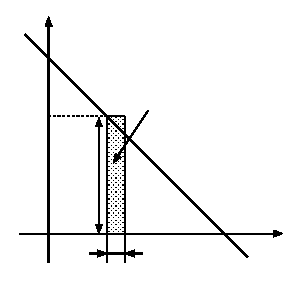
\includegraphics{int_triangle.eps}}}
%    \begin{overpic}[width=4.5cm,grid,tics=10]{int_triangle.eps}
    \begin{overpic}[width=4.5cm]{int_triangle.eps}
      {\small
        \put(5,5){$O$}
        \put(90,7){$x$}
        \put(5,90){$y$}
        \put(74,5){$1$}
        \put(6,74){$1$}

        \put(27,7){$x$}
        \put(42,7){$x+dx$}
        \put(33,-3){$dx$}
        \put(4,55){$y$}
        \put(24,28){\rotatebox{90}{$1-x$}}
        \put(48,62){$dS=dx\cdot (1-x)$}
%        \put(60,85){$y=f(x)=1-x$}
      }
    \end{overpic}
  }
  \subcaptionbox{}{
%    \resizebox{4.5cm}{!}{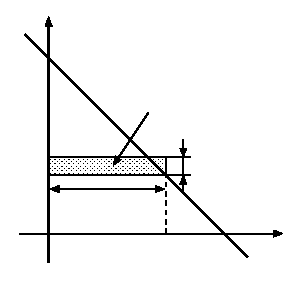
\includegraphics{int_triangle2.eps}}}
%    \begin{overpic}[width=4.5cm,grid,tics=10]{int_triangle2.eps}
    \begin{overpic}[width=4.5cm]{int_triangle2.eps}
      {\small
        \put(5,5){$O$}
        \put(90,7){$x$}
        \put(5,90){$y$}
        \put(78,15){$1$}
        \put(6,74){$1$}

%        \put(53,6){$x$}
        \put(24,23){$1-y$}
        \put(53,6){$x$}
%        \put(56,0){$=(1-y)$}
        \put(6,32){$y$}
        \put(-11,40){$y+dy$}
        \put(68,35){$dy$}
        \put(48,60){$dS=dy\cdot (1-y)$}
%        \put(60,85){$x=g(y)=1-y$}
      }
    \end{overpic}
  }
  \subcaptionbox{}{
%    \resizebox{4.5cm}{!}{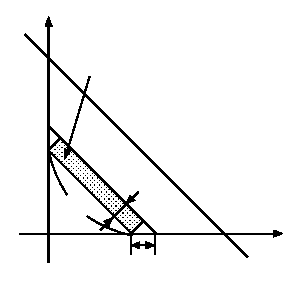
\includegraphics{int_triangle3.eps}}}
%    \begin{overpic}[width=4.5cm,grid,tics=10]{int_triangle3.eps}
    \begin{overpic}[width=4.5cm]{int_triangle3.eps}
      {\small
        \put(5,5){$O$}
        \put(90,7){$x$}
        \put(5,90){$y$}
        \put(74,5){$1$}
        \put(6,74){$1$}
        \put(36,6){$x$}
        \put(43,0){$dx$}
        \put(39,28){\rotatebox{45}{$\frac{dx}{\sqrt{2}}$}}
       \put(13,27){\rotatebox{315}{$\sqrt{2}x$}}
        \put(20,75){$dS=\sqrt{2}x\cdot\frac{dx}{\sqrt{2}}$}
%        \put(60,85){$t=h(s)=2s$}
      }
    \end{overpic}
  }
  \subcaptionbox{}{
%    \resizebox{4.5cm}{!}{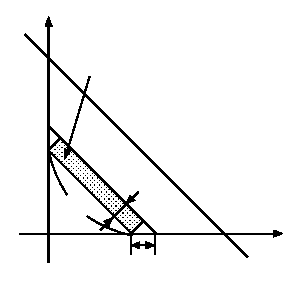
\includegraphics{int_triangle3.eps}}}
%    \begin{overpic}[width=4.5cm,grid,tics=10]{int_triangle3.eps}
    \begin{overpic}[width=4.5cm]{int_triangle4.eps}
      {\small
        \put(5,5){$O$}
        \put(90,7){$x$}
        \put(5,90){$y$}
        \put(74,5){$1$}
        \put(6,74){$1$}

        \put(26,21){\rotatebox{45}{$s$}}
        \put(33,29){\rotatebox{45}{$s+ds$}}
        \put(38,51){\rotatebox{45}{$\frac{1}{\sqrt{2}}$}}
        \put(49,2){\rotatebox{45}{$ds$}}
 %       \put(15,18){$h(s)$}
       \put(17,23){\rotatebox{315}{$2s$}}
        \put(20,75){$dS=ds\cdot 2s$}
        \put(62,57){\rotatebox{45}{$s$}}
        \put(-3,17){\rotatebox{45}{$t$}}
%        \put(60,85){$t=h(s)=2s$}
      }
    \end{overpic}
  }
    \caption{三角形の面積を求める。(a) $x$軸に沿って分割。(b) $y$軸に
      沿って分割。
      (c) $x$軸方向に分割して,斜辺と平行な長方形に注目。(d) 斜辺と垂
      直な軸に沿って分割して,斜辺と平行な長方形に注目。}
    \label{fig:int_triangle}
  \end{center}
\end{figure}

もう一度面積と定積分の関係を復習するために,
次式で表される三角形の面積を求めてみよう。
\begin{align}
  \begin{cases}
x&\ge 0\\
y&\ge 0\\
y&\le -x+1
  \end{cases}\label{eq:S-triangle}
\end{align}

求める面積は,図\ref{fig:int_triangle}(a)で示すように
底辺のある位置$x$での微小長さ$dx$ およびその点での高さ$f(x)=-x+1$の積
である微小面積$dS=dx\cdot f(x)$を$0\le x\le 1$の範囲で足し合わせ,
すなわち次式で与えられる。
\begin{align}
  \int_{三角形内} dS &= \int_0^1 dx\cdot f(x)\notag\\
  &=  \int_0^1(1-x)dx \notag\\
  &=  -\int_0^1(x-1)dx \notag\\
  & = -\left.\frac{(x-1)^2}{2}\right|_0^1\notag\\
  & = \frac{1}{2}\notag\notag
\end{align}
% このように,まず微小な面積を$dx$を用いて表して,それを積分するこ
% とによって全体の面積を求めることができる。
\question
式(\ref{eq:S-triangle})の面積を以下の方法で求めなさい
\answer{
(\ref{item:S-triangle-dy}) $\displaystyle S=\int_0^1(1-y)dy$~
(\ref{item:S-triangle-dx2}) $\displaystyle S=\int_0^1\sqrt{2}x\cdot\frac{dx}{\sqrt{2}}$~
(\ref{item:S-triangle-ds}) $\displaystyle S=\int_0^{\frac{1}{\sqrt{2}}}2sds$~
}。
\begin{enumerate}
\item\label{item:S-triangle-dy} $y$軸方向に微小領域を分割して積分計算
  をする
  (図\ref{fig:int_triangle}(b))。
\item\label{item:S-triangle-dx2}  $x$軸方向に微小領域を分割するが,
  斜辺と平行な長方形に着目して積分計算をする (図\ref{fig:int_triangle}(c))。
\item\label{item:S-triangle-ds}  斜辺と直交する方向に微小領域を分割し
  て積分計算をする (図\ref{fig:int_triangle}(d))。
\end{enumerate}

\begin{figure}[t]
  \centering
  \subcaptionbox{}{
%    \resizebox{4.0cm}{!}{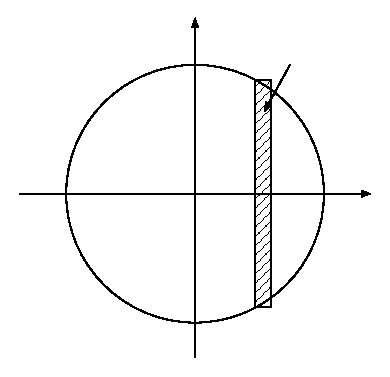
\includegraphics{circle-xy.eps}}}
%    \begin{overpic}[width=4.5cm,grid,tics=10]{circle-xy.eps}
    \begin{overpic}[width=4.5cm]{circle-xy.eps}
      {\small
        \put(40,40){$O$}
        \put(95,41){$x$}
        \put(44,94){$y$}
        \put(87,42){$a$}
        \put(3,42){$-a$}
        \put(45,85){$a$}
        \put(38,5){$-a$}

        \put(60,49){$x$}
        \put(73,49){$x+dx$}
%        \put(66,68){$dx$}
        \put(57,85){$dS=2\sqrt{a^2-x^2}\cdot dx$}
      }
    \end{overpic}
  }
  \subcaptionbox{}{
%    \resizebox{4.0cm}{!}{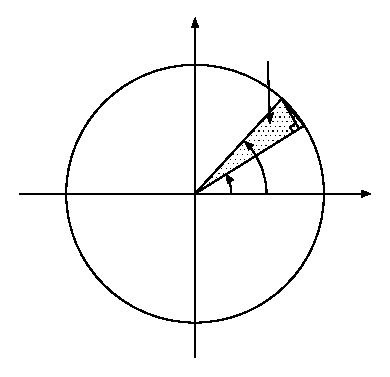
\includegraphics{circle-r.eps}}}
%    \begin{overpic}[width=4.5cm,grid,tics=10]{circle-r.eps}
    \begin{overpic}[width=4.5cm]{circle-r.eps}
      {\small
        \put(40,40){$O$}
        \put(95,41){$x$}
        \put(44,94){$y$}
        \put(87,42){$a$}
        \put(3,42){$-a$}
        \put(45,85){$a$}
        \put(38,5){$-a$}

        \put(62,50){$\theta$}
       \put(72,50){$\theta+d\theta$}
%        \put(66,68){$d\theta$}
        \put(57,85){$dS=\frac{1}{2}a\cdot ad\theta$}
      }
    \end{overpic}
  }
  \subcaptionbox{}{
%    \begin{overpic}[width=4.5cm,grid,tics=10]{circle-r2.eps}
    \begin{overpic}[width=4.5cm]{circle-r2.eps}
      {\small
        \put(40,40){$O$}
        \put(95,41){$x$}
        \put(44,94){$y$}
        \put(87,42){$a$}
        \put(3,42){$-a$}
        \put(45,85){$a$}
        \put(38,5){$-a$}

        \put(78,80){$r$}
        \put(65,55){$r$}
        \put(72,60){$r+dr$}
%        \put(64,68){$dr$}
        \put(-7,85){$dS=2\pi r\cdot dr$}
      }
    \end{overpic}
  }
  \caption{円の面積を求める。(a)直交座標で。(b)極座標で。(c)極座標で
    (その2)。}
  \label{fig:S-circle}
\end{figure}

\begin{figure}[h]
  \begin{center}
    \resizebox{5cm}{!}{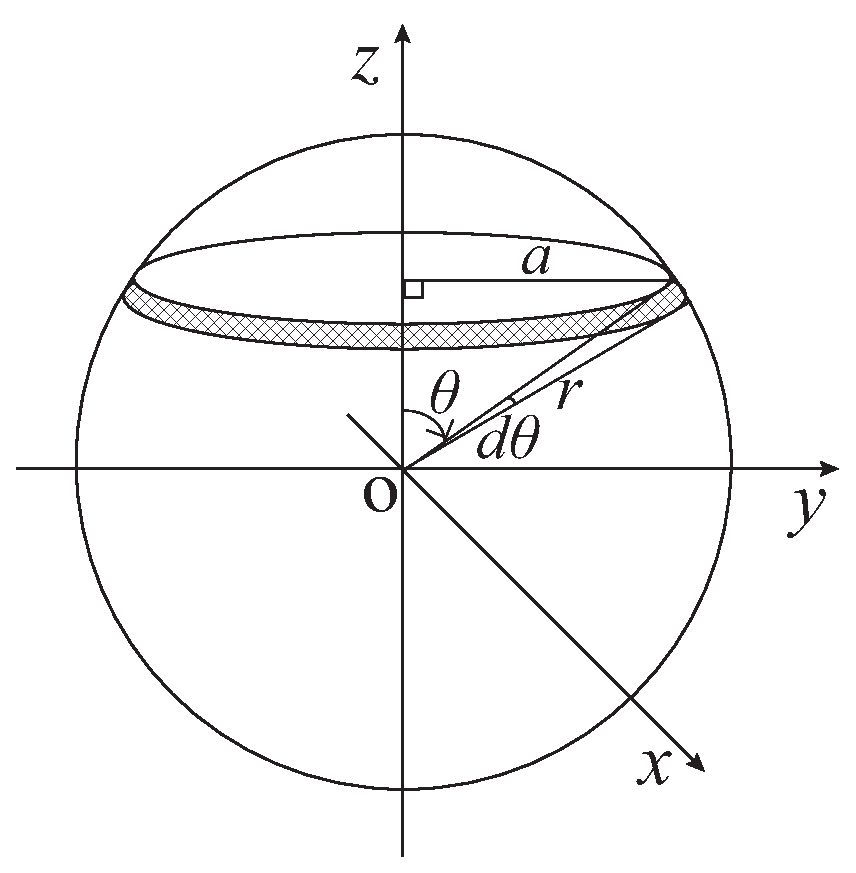
\includegraphics{Ssphere.eps} }
    \caption{\label{fig:Ssphere}
      球の表面積を求める方法例}
  \end{center}
\end{figure}

\exercise
以下の各面積を積分計算を用いて求めなさい。
どのように考えて計算式を導いたかは図示して説明すること。
可能なものは幾何学的方法でも面積を求めなさい
\answer{
(\ref{item:S:y=x}) $\displaystyle\int_1^2xdx$~
(\ref{item:S:y=x^2+1}) $\displaystyle\int_2^3(x^2+1)dx$~
(\ref{item:S:y=(x^2+1)dy}) $\displaystyle 2\int_2^3\sqrt{y-1}dy$\\
(\ref{item:S:circle}) (a) $\displaystyle 2\int_{-a}^a\sqrt{a^2-x^2}dx$~
(b) $\displaystyle \int_0^{2\pi}\frac{1}{2}a\cdot ad\theta$~
(c) $\displaystyle \int_0^a2\pi rdr$ ~
(\ref{item:S:cylinder}) $\displaystyle\int_0^h2\pi rdh$~or
$\displaystyle\int_0^{2\pi}hr d\theta$
(\ref{item:S:sphere})$\displaystyle\int_0^{\pi} 2\pi r\sin\theta
\cdot rd\theta$
}。
\begin{enumerate}
\item\label{item:S:y=x} 直線$y=x$, $x=1$, $x=2$, $x$軸で囲まれた領域
\item\label{item:S:y=x^2+1} 曲線$y=x^2+1$, $x=2$, $x=3$, $x$軸で囲まれた領域
\item\label{item:S:y=(x^2+1)dy} 曲線$y=x^2+1$, $y=2$, $y=3$で囲まれた領域
\item\label{item:S:circle} 半径$a$の円の面積
  \begin{enumerate}
  \item 直交座標による積分で(図\ref{fig:S-circle}(a))
  \item 極座標の偏角方向の積分で(図\ref{fig:S-circle}(b))
  \item 極座標の動径方向の積分で(図\ref{fig:S-circle}(c))
  \end{enumerate}
\comment この問により,円の面積$\pi r^2$の微分が円周$2\pi r$を与える理
由がわかる。
正方形等も,中心から各辺までの距離$s$を用いて面積を表せば,その微分は
周の長さになる。
% \item\label{item:S:cylinder} 半径$r$, 高さ$h$の円柱の側面の表面積
\item\label{item:S:sphere} 半径$r$の球の表面積(図\ref{fig:Ssphere})
\end{enumerate}

\subsubsection{体積}
\begin{figure}[t]
  \begin{center}
    \resizebox{4.5cm}{!}{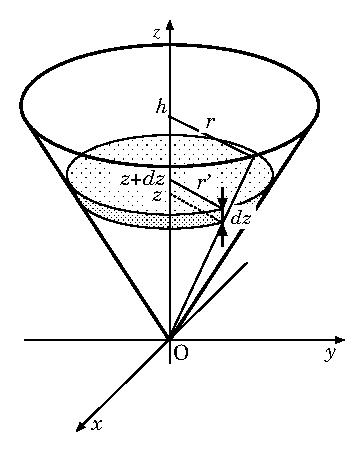
\includegraphics{cone.eps}}
    \caption{円錐の体積}
    \label{fig:cylinder}
  \end{center}
\end{figure}
\nmindex[たいせき]{体積}(\nmindex{Volume})の計算も面積の場合と同様に,
まず微小な体積を$dx$を用いて表して,それを積分することによって求めることができる。

例えば,底面が半径$r$の円であり高さが$h$の円錐の体積を求めてみよう。
計算を簡単にするためこの円錐を逆さにし,
その頂点を原点に,$z$軸が円錐の中心軸と一致するようにとる(図\ref{fig:cylinder})。

この円錐の微小高さ$z\sim z+dz$における微小部分の体積を半径
$\displaystyle r'=\frac{z}{h}r$,
高さ$dz$の微小円柱と同じとみなすと、その体積$dV$は次式で与えられる。
\begin{align}
dV=dz\cdot\pi r'^2=dz\cdot\pi\left(\frac{z}{h}r\right)^2\notag
\end{align}
よって体積$V$は次式で与えられる。
\begin{align}
  V&=\int_{円錐全体} dV\notag\\
  &=\int_0^hdz\cdot\pi r'^2\notag\\
  &=\int_0^hdz\cdot\pi\left(\frac{z}{h}r\right)^2\notag\\
%   &=\pi\left(\frac{r}{h}\right)^2\int_0^hz^2dz\notag\\
  &=\frac{1}{3}\pi r^2h\notag
\end{align}

% \begin{figure}[h]
%   \begin{center}
%     \resizebox{4.5cm}{!}{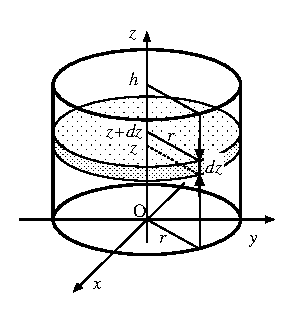
\includegraphics{cylinder.eps}}
%     \caption{円筒の体積}
%     \label{fig:cylinder}
%   \end{center}
% \end{figure}
% 体積の計算も面積の場合と同様に,まず微小な体積を$dx$を用いて表して,そ
% れを積分することによって求めることができる。

% 例えば,底面が半径$r$の円であり高さが$h$の円筒の体積を求めてみよう。
% 図\ref{fig:cylinder}のように,$z$軸が円筒の中心軸と一致するようにとり,
% 底面を$xy$平面上にとる。この円筒の微小高さ$z\sim z+dz$における微小体積
% は$dz\cdot\pi r^2$。よって体積$V$は次式で与えられる。
% \begin{align}
%   V=\int_0^hdz\cdot\pi r^2=\pi r^2z|_0^h=\pi r^2h\notag
% \end{align}

\begin{figure}[t]
  \begin{center}
    \resizebox{5cm}{!}{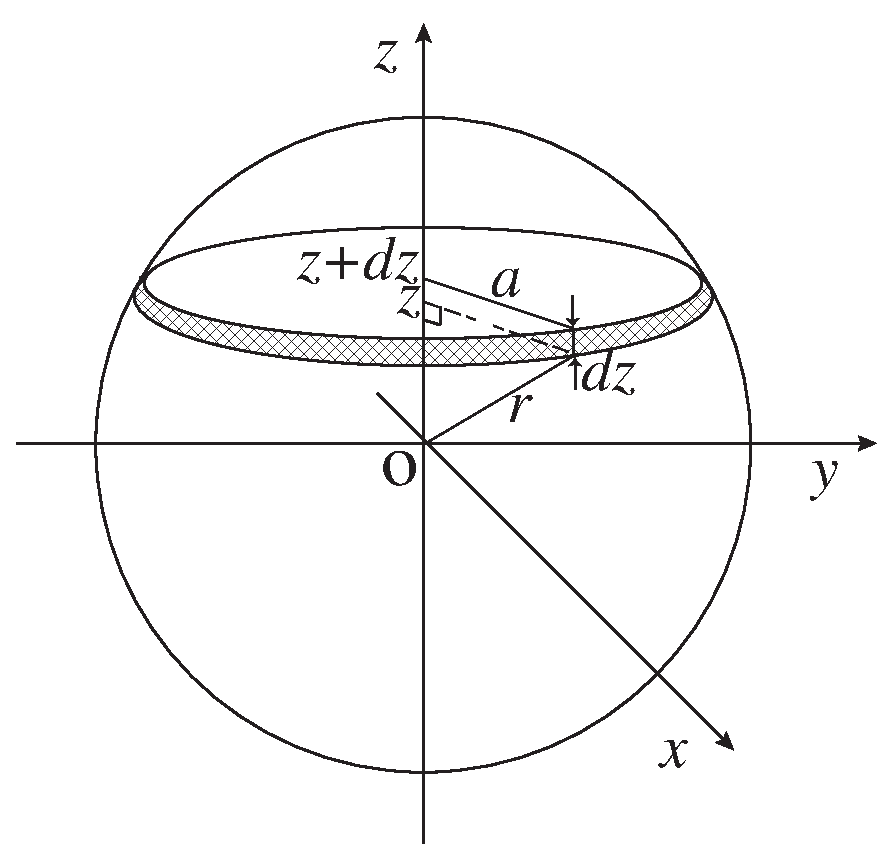
\includegraphics{Vsphere.eps} }
    \caption{\label{fig:Vsphere}
      球の体積を求める方法例}
  \end{center}
\end{figure}

\question
以下の立体の体積を求めなさい。
どのように計算式を導いたかを図を描いて説明すること。
\begin{enumerate}
% \item 底面が半径$r$の円であり高さが$h$の円錐
\item 半径$r$の球
  \begin{enumerate}
  \item 半径$a$の球の表面積を$S(a)$とおいて求める。
  \item 上記以外の方法で求める(例えば,図\ref{fig:Vsphere}参照)。
  \end{enumerate}
\item 底面が一辺の長さ$r$の正方形であり高さが$h$の四角錐
\end{enumerate}
\comment 上問の(1)の(a)により,球の体積$\frac{4}{3}\pi r^3$の微分が球
の表面積$4\pi r^2$を与える理由がわかる。
立方体等も,中心から各辺までの距離$s$を用いて体積を表せば,その微分は
表面積になる。

\subsubsection{曲線の長さ}
\begin{figure}[h]
  \begin{center}
    \resizebox{5cm}{!}{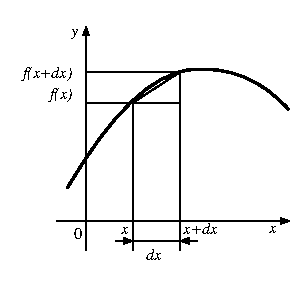
\includegraphics{int_line.eps} }
    \caption{線分の長さを求める}
    \label{fig:int_line}
  \end{center}
\end{figure}

2次元空間内の曲線$y=f(x)$, $x\in[a,b]$の長さを知りたいとき,
どのように計算すればよいか考えてみよう。
関数$y=f(x)$は区間$x\in[a,b]$で微分可能であるとする。

微小区間[$x,x+dx$]における曲線の長さ$dl$は
%$dy=f(x+dx)-f(x)$とおくと
次式で与えられる(図\ref{fig:int_line}参照)。
\begin{align}
  dl
  &=\sqrt{(dx)^2+(f(x+dx)-f(x))^2}\notag\\
  &=dx\sqrt{1+\left(\frac{f(x+dx)-f(x)}{dx}\right)^2}\notag
%  &=\sqrt{(dx)^2+(dy)^2}\notag\\
%  &=dx\sqrt{1+\left(\frac{dy}{dx}\right)^2}\notag
\end{align}
よって,$dx$が十分小さいとき
\begin{align}
  dl\simeq dx\sqrt{1+(f'(x))^2}\notag
\end{align}
となる。
求める曲線の長さ$l$は$dl$を区間[$a,b$]で全て足しあわせたものな
ので,次式で与えられる。
\begin{align}
  l=\int_{曲線上} dl=\int_a^b dx\sqrt{1+(f'(x))^2}\notag
\end{align}

\exercise
以下の長さを積分計算により求めなさい
\answer{
(\ref{item:hcos}) $e-e^{-1}$,
(注) $y=\frac{a}{2}(e^{\frac{x}{a}}+e^{-\frac{x}{a}})$は糸の両端を持っ
て垂らしたときにできる曲線(懸垂線)を表す。
}。
\begin{enumerate}
\item $y=x$の区間$x\in[0,1]$における長さ
\item 円周の長さ
\item \label{item:hcos}$\displaystyle y=\frac{e^x+e^{-x}}{2}$の区間
  $x\in[-1,1]$における長さ
%% \item 3次元円筒座標で次式で表される線分の長さ
%%   \begin{align}
%%     \begin{cases}
%%       r=1\\
%%       \theta=z,\quad z\in[0, 2\pi]
%%     \end{cases}\notag
%%   \end{align}
\end{enumerate}

\subsection{広義積分}

積分区間の一端(もしくは両端)で被積分関数が発散する場合や,
積分区間の一端(もしくは両端)が正もしくは負の無限大となる定積分を
\bfindex[こうぎせきぶん]{広義積分}と呼ぶ。
例えば, 以下の定積分を考えよう。
\begin{align}
  \int_0^{\infty}e^{-x}dx\notag
\end{align}
この積分値は次のように定義される。
\begin{align}
  \lim_{a\to \infty}\int_0^{a}e^{-x}dx\notag
\end{align}

\question
以下の計算をし,出来るだけ簡単な形で答えなさい
\answer{
(\ref{eq:int2:e^(-x)}) $1$~
(\ref{eq:int2:x^(-2/3)}) $3$
% (\ref{eq:int2:1/x^2}) $\infty$
% (\ref{eq:int2:dx/(1-x)}) $-1$~
%(\ref{eq:int2:(logx)^2dx}) $e$~
}。
\begin{enumerate}
\item\label{eq:int2:e^(-x)}   $\displaystyle\int_0^{\infty}e^{-x}dx$
\item\label{eq:int2:x^(-2/3)}   $\displaystyle\int_0^1\frac{dx}{x^{\frac{2}{3}}}$
% \item\label{eq:int2:1/x^2}   $\displaystyle\int_0^1\frac{1}{x^2}dx$
% \item\label{eq:int2:dx/(1-x)} $\displaystyle\int_1^{e+1}\frac{1}{1-x}dx$%=\qbox[$-1$]$
%\item\label{eq:int2:(logx)^2dx} $\displaystyle \int_0^e (\log x)^2 dx$%=\qbox[$2$]$
\end{enumerate}

\subsection{力学と微積分}

%%%%%%%%%%%%%%%%%%%%%%%%%%%%%%%%5
\subsubsection{重心と積分}

%%%%%%%%%%%%%%%%%%%%%%%%%%%%%%%%5
\nquestion
長さ$l$, 質量$m$の棒がある。
この棒に沿って$x$軸を取り, その原点は棒の一端にとる。
この棒は位置によって線密度(単位長さあたりの質量)が異なる。
そこで位置$x$における線密度を$\rho(x)$とおく。
この棒について以下の問に答えなさい
\answer{
(\ref{item:stick-m})~$\displaystyle m=\int_0^l\rho(x)dx$\\
(\ref{item:stick-com})~$\displaystyle X=\frac{\displaystyle\int_0^lx\rho(x)dx}{\displaystyle\int_0^l\rho(x)dx}=\frac{1}{m}\int_0^lx\rho(x)dx$\\
(\ref{item:stick-com-1})~$\displaystyle X=\frac{l}{2}$,
(線密度は(\ref{item:stick-m})の関係式を用いると$\rho=m/l$)\\
(\ref{item:stick-com-2})~$\displaystyle X=\frac{2}{3}l$,
(線密度は$\displaystyle\rho=\frac{2m}{l^2}x$)
}。
\begin{enumerate}
\item\label{item:stick-m} $\rho(x)$と$m$の関係式を表しなさい。
\item\label{item:stick-com} この棒の重心位置$X$を表す式を書きなさい
  \footnote{質量$m_1, m_2, \cdots, m_n$の物体がそれぞれ位置$x_1, x_2,
    \cdots, x_n$にあるとき,
    その重心位置$X$は
    $\displaystyle X=\frac{\displaystyle\sum_{i=1}^nm_ix_i}{\displaystyle\sum_{i=1}^nm_i}$で与えられる。
  }。
\item\label{item:stick-com-1} 線密度$\rho$が実は位置によらない定数であっ
  た場合について重心位置を求めなさい。ただし, $\rho$を使わずに答えること。
\item\label{item:stick-com-2} 線密度が$\rho(x)$が原点からの距離に比例
  する場合について重心位置を求めなさい。ただし, $\rho$を使わずに答えること。
\end{enumerate}

%\subsubsection{距離・速度・加速度}
%\question
%ある物体が直線上を運動している。
%この物体は時刻$t=0$ [s] には原点にあったが,$0\le t\le 3$ [s]の間
%$a=2$ [m$/$s$^2$]の等加速度運動を行った後,$a=-1$ [m$/$s$^2$]の等加速
%度運動に移行し、時刻$t_f$に原点に戻ってきた
%\answer{
%物体の位置を$x$座標で表すと
%(\ref{item:xva-xv})~ $\dot{x}(3\mbox{[s]})=6$ m$/$s~,\\ $x(3\mbox{[s]})=9$ [m]~
%(\ref{item:xva-t})~ $t_f=9+3\sqrt{6}$ [s]
%}
%。
%\begin{enumerate}
%\item\label{item:xva-xv} $t=3$ [s]における物体の速度と位置を求めなさい。
%\item\label{item:xva-t} 物体が原点に戻ってきた時刻$t_f$を求めなさい。
%\item\label{item:xva-graph} $t=0$から$t_f$までの物体の速度変化のグラフ
%  を書き,$t_f$とはどのような時刻かについて幾何学的に説明しなさい。
%\end{enumerate}

\subsubsection{運動量・力積・運動エネルギー・仕事}

\nquestion
質量$m$の物体の位置を$x$座標を用いて表す。
物体に一定の力$F$が$x$座標の正の方向に働くときの運動方程式は次式で与え
られる。
\begin{align}
  m\ddot{x}=F\notag
\end{align}
$v=\dot{x}$とおくと次式をえる。
\begin{align}
  m\dot{v}=F\notag
\end{align}
\begin{enumerate}
\item $F$が常に0の場合,$v$は時間とともにどのように変わるか。
  $v$の微分は$v$の時間変化率を表す事に注意して$v$の時間変化の
  グラフを書いて説明しなさい。
\item $F$が一定値の場合,その符号に応じて$v$は時間とともにどのように変
  わるか。グラフを書いて説明しなさい。
\item
物体が力$F(t)$をうけながら時刻$t$から$t+\Delta t$までの間に$x$から
$x+\Delta x$まで移動した。
このとき以下の式が成立することを証明しなさい。
\begin{enumerate}
\item 運動量と力積の関係式
\begin{align}
  mv(t+\Delta t)&-mv(t)=\int_t^{t+\Delta t}Fdt\notag\\
  =&F\Delta t\quad (F: 一定のとき)\notag
\end{align}
\item 運動エネルギーと仕事の関係式
\begin{align}
  \frac{1}{2}mv^2(t+\Delta t)&-\frac{1}{2}mv^2(t)=\int_x^{x+\Delta x}Fdx\notag\\
  =&F\Delta x\quad (F: 一定のとき)\notag
\end{align}
\end{enumerate}
\end{enumerate}

\newpage
\section{微分方程式}

未知関数とその導関数を含む方程式を\bfindex[びぶんほうていしき]{微分方程式}とよぶ。微分方程式を満たす未知関数を\textbf{微分方程式の解}とよぶ。方程式の解は未知変数の値であるが,\textbf{微分方程式の解は関数}である。

\subsection{微分方程式の解の挙動}
\nquestion
$\dot{x}>0$の場合,$x$は時間とともに増えるだろうか,それとも減る
だろうか。$|\dot{x}|$の大きさにより,$x$の時間変化の割合はどのように変
わるだろうか。
理由とともに述べなさい。
%% 微分方程式$\dot{x}=-x$の解の軌跡を,横軸を時刻$t$, 縦軸を$x$として
%%   図示せよ(\textbf{解を求めずに}グラフを考える)。
%%   また解を求め,先に図示した軌跡と一致することを確認せよ。

\nquestion
以下の各微分方程式の解の挙動をグラフに表しなさい。
\begin{enumerate}
\item $\dot{x}=x$
\item $\dot{x}=1-x$
  % \item $\dot{x}=\sin x$
\item $\dot{x}=(1-x)x$
% \item $y'=y^2-3y+2$
\end{enumerate}


\subsection{変数分離型微分方程式の解法}
以下の微分方程式の解を求めよ。また,求めた解を微分方程式に代入す
ることにより検算せよ
\answer{
(\ref{item:dx=x}) $x=Ce^t$
(\ref{item:dx=1-x}) $x=Ce^{-t}+1$
(\ref{item:dx=x(1-x)}) $x=\frac{1}{1-Ce^{-t}}$
(\ref{item:dy+ay}) $y=Ce^{-ax}$~
(\ref{item:dy-xy}) $y=Ce^{\frac{1}{2}x^2}$~
(\ref{item:dv+av-b}) $v=\frac{b}{a}+Ce^{-at}$~
(\ref{item:dy-x(1-y)}) $y=1+C e^{-\frac{1}{2}x^2}$
(\ref{item:dy-4x3y}) $y=Ce^{x^4}$
 (\ref{item:dy+ytanx}) $y=C\cos x$
% (\ref{item:dx-sinx}) $\tan\frac{x}{2}=Ce^t$
% (\ref{item:dx-(a-bx)x}) $x=\frac{a}{b}\frac{1}{1-Ce^{-at}}$
% (\ref{item:yydy+xy3-x}) $y=\sqrt[3]{1+Ce^{-\frac{3}{2}x^2}}$
% (\ref{item:dysqrt(x-1)-sqrt(y-1)}) $\sqrt{y-1}=\sqrt{x-1}+C$, $y=1$
}。
\begin{enumerate}
\item \label{item:dx=x}$\dot{x}=x$
\item \label{item:dx=1-x} $\dot{x}=1-x$
\item \label{item:dx=x(1-x)} $\dot{x}=x(1-x)$
\item \label{item:dy+ay}$y'=-ay$, ($a:$ 定数)
\item \label{item:dy-xy}$y'=xy$
\item \label{item:dv+av-b}$\dot{v}=-av+b$, \quad($a,b:$ 定数)
\item \label{item:dy-x(1-y)}$y'=x(1-y)$
\item \label{item:dy-4x3y}$y'-4x^3y=0$
\item \label{item:dy+ytanx}$y'+y\tan x=0$
% \item \label{item:dx-sinx}$\dot{x}=\sin x$
% \item \label{item:dx-(a-bx)x}$\dot{x}=(a-bx)x$, \quad($a,b:$ 定数)
% \item \label{item:yydy+xy3-x}$y^2y'+xy^3=x$
% \item \label{item:dysqrt(x-1)-sqrt(y-1)}$y'\sqrt{x-1}-\sqrt{y-1}=0$
\end{enumerate}


\subsection{微積分と定性的表現}

% %%%%%%
% \nquestion
% 木などの有機物中に閉じ込められた炭素14は時間とともに崩壊して
% 窒素14に変化していく。
% その崩壊の速度(炭素14の量の時間変化率)は, 炭素14の量に比例することが知
% られている\answer{
% (1) $\dot{N}=-aN$, $a$は正の定数。\quad
% (2 )$N=N_0\left(\frac{1}{2}\right)^{\frac{t}{\tau}}$,
%   $N_0$は$t=0$における炭素14の量。
% }。
% \begin{enumerate}
% \item ある時間$t$ [年]における炭素14の量を$N(t)$とおく。
%   $N(t)$の時間変化を表す微分方程式を書きなさい。
% \item 炭素14の半減期は$\tau=5730$年である。
%   このとき, 前問の微分方程式を解いて$N(t)$を表す式を導きなさい。
% \end{enumerate}

%%%%%%
\nquestion 放射性物質の量は時間とともに減少し,その時間変化率は常にその
時の物質量に比例する。このとき,下記の問いに答えなさい\answer{
(1) $\dot{n}=-an$, $a$は正の定数。\quad
(2) $n=Ce^{-at}$\quad
(3) $n=n_0\left(\frac{1}{2}\right)^{\frac{t}{\tau}}$,
  $n_0$は$t=0$における放射性物質の量。
(4) $2.01\times 10^2$年}。
% \begin{align}
%   n(t)=n_0\left(\frac{1}{2}\right)^{\frac{t}{30}}\notag
% \end{align}
% ここで, $n_0$は$t=0$における物質量である。
\begin{enumerate}
\item ある放射性物質の時刻$t$における量を$n(t)$とする。$n(t)$が満たす
  べき微分方程式を書きなさい。
\item 前問の微分方程式を解き,$n(t)$を時間の関数として表しなさい。
\item この物質の半減期を$\tau$とおく。前問で求めた$n(t)$を$\tau$を用い
  た出来るだけ簡単な表現に書き直しなさい。
\item 放射性同位体であるセシウム137の半減期は$30.2$年である。
% \item $t_{100}$を求めるために解くべき方程式を$n(t), n(t+t_{100})$と数値のみを
%   用いて書きなさい。
%   \aline[$\displaystyle\frac{1}{100}n(t)=n(t+t_{100})$]{7cm}
  セシウム137の量が元の1/100になるまで何年かかるかを求めなさい。
  必要なら$\log_25=2.322$を使い,有効数字3桁で答えなさい。
\anscomment{
      \begin{align}
        n(t+t_{100})&=\frac{1}{100}n(t)\notag\\
        C\cdot 2^{-\frac{t+t_{100}}{\tau}}
        &=\frac{1}{100}\cdot C\cdot 2^{-\frac{t}{\tau}}\notag\\
        2^{-\frac{t_{100}}{\tau}}&=\frac{1}{100}\notag\\
        -\frac{t_{100}}{\tau}&=\log_2\frac{1}{100}\notag\\
        t_{100}&=\tau\log_2{100}\notag\\
        &=30.2[yr]\times 2\times \log_2{10}\notag\\
        &=30.2[yr]\times 2\times (1+2.322)\notag\\
        &=200.6[yr]=2.01\times 10^2[yr]\notag
\end{align}}
\end{enumerate}

%%%%%%
\nquestion
以下の問に答えなさい
\answer{
(\ref{item:bucket}) 積分方程式は$\displaystyle V=\int_0^tadt$,
微分方程式は$\dot{V}=a$。ただし$V(0)=0$。
(\ref{item:bucket-hole})
積分方程式は$\displaystyle V=b-\int_0^tkVdt$ ($k$は正の定数)。
微分方程式は$\displaystyle \dot{V}=-kV$ ($k$は正の定数)。ただし,$V(0)=b$.
(\ref{item:bucket-in-out})
積分方程式は$\displaystyle V=\int_0^t(a-kV)dt$ ($k$は正の定数)
微分方程式は$\displaystyle \dot{V}=a-kV$ ($k$は正の定数)。ただし,$V(0)=0$.
(\ref{item:bucket-final}) 前問の微分方程式において$\dot{V}=0$となる時
の$V$が求める値。すなわち,$V=a/k$。微分方程式の解を求めて
$\displaystyle\lim_{t\to\infty}V(t)$を求めても良い。
}。
\begin{enumerate}
\item\label{item:bucket} 空のバケツに毎秒$a$リットルの水を入れる。入れ
  始めてから$t$秒後の水の量を$V(t)$を定積分を使って表しなさい。
  また,$V$が満たすべき微分方程式を書きなさい。
\item\label{item:bucket-hole} バケツにはじめ$b$リットルの水が入れたが,
  底に小さな穴があいていて水が少しずつ漏っていた。
  単位時間あたりに水の漏る量はバケツに残っている水の量$V$に比例することがわかった。
  バケツに水を入れてから$t$秒後の水の量$V$とする。
  上記の文章を定式化することにより,
  $V$が満たすべき積分方程式と微分方程式をそれぞれ書きなさい。
\item\label{item:bucket-in-out}
  空のバケツに毎秒$a$リットルの水を入れる。
  しかし, このバケツには小さな穴が空いていて水が漏る。
  単位時間あたりに水の漏る量はバケツに残っている水の量$V$に比例する。
  バケツに水を入れ初めてから$t$秒後の水の量を$V$とするとき,
  $V$が満たすべき積分方程式と微分方程式をそれぞれ書きなさい。
\item\label{item:bucket-final} 前問のバケツにしばらく水を入れ続けてい
  るとやがてバケツの水の量が変化しなくなった。
  $a$は定数であったとして, このときの水の量$V$を求めなさい。
\end{enumerate}

\nquestion
落下する雨粒には,その速度に比例した働く粘性抵抗と重力が働く。
雨粒の運動方程式を書き,十分時間がたったときの速度を求めなさい。

\subsection{斉次線形微分方程式の解法}

未知関数とその導関数(高階導関数を含む)の線形和のみを含む微分方程式を,
\bfindex[せいじせんけいびぶんほうていしき]{斉次線形微分方程式}とよぶ。


以下の二階斉次線形微分方程式の解を求めよう。
\begin{align}
  \label{eq:2diffeq}
  \ddot{x}+a\dot{x}+bx=0
\end{align}
\begin{enumerate}
\item 微分方程式の解を$x=Ce^{\lambda t}$と仮定し,実際にこれが式
  (\ref{eq:2diffeq})の解となるには$\lambda$がどのような条件を満たせ
  ばよいかを議論しなさい。

  \comment
  $x=Ce^{\lambda t}$が式(\ref{eq:2diffeq})の解となるために$\lambda$が
  満たすべき方程式を\bfindex[とくせいほうていしき]{特性方程式}という。
\item 特性方程式の解を$\lambda_1$, $\lambda_2$とすると,
  微分方程式の解は次のようになることを示しなさい。
  \begin{enumerate}
  \item $\lambda_1\ne\lambda_2$の時
    \begin{align}
      x=C_1e^{\lambda_1t}+C_2e^{\lambda_2t}\notag
    \end{align}
    ただし,$\lambda=\alpha\pm i\omega$, ($\omega\ne 0$)の場合には
    以下のように書けることを示しなさい。
    \begin{align}
      x=e^{\alpha t}(C_1\cos{\omega t}+C_2\sin{\omega t})\notag
    \end{align}
  \item $\lambda_1=\lambda_2$の時
    \begin{align}
      x=(C_1+C_2t)e^{\lambda_1t}\notag
    \end{align}
  \end{enumerate}
\item 解の振舞を$a$, $b$の値によって分類し,図示して説明しなさい。
\end{enumerate}

\nquestion
水平面上に質量を無視できるバネを置き,一端は壁に,もう一端には質量$m$の重りをつけた。その後,重りを少し引っ張ってから手を離し,重りの運動を観察した。
 重りと床面の間には粘性摩擦(速度に比例する大きさの抵抗力)がはたらくが,静止摩擦や動摩擦は働かないものとする。バネ定数を$k$, 粘性摩擦係数を$\sigma$とする。
\begin{enumerate}
	\item 重りの運動方程式を書きなさい。
	\item バネ定数や粘性摩擦係数が変化するとバネの運動がどのように変化しうるか説明しなさい。
\end{enumerate}


\exercise
以下の微分方程式の解をそれぞれ求め,解軌道を図示しなさい。
また,求めた解を微分方程式に代入することにより検算をしなさい
\answer{
(1) $y=e^{-x}-e^{-5x}$~
(2) $y=\sin 2x$~
(3) $y=(x+2)e^{2x}$~
(4) $x=2e^{-2t}(\cos t+2\sin t)$~
}。
\begin{enumerate}
\item $y''+6y'+5y=0$, $y(0)=0$, $y'(0)=4$
\item $y''+4y=0$, $y(0)=0$, $y'(0)=2$
\item $y''-4y'+4y=0$, \;$y(0)=2$, \;$y'(0)=5$
\item $\ddot{x}+4\dot{x}+5x=0$, $x(0)=2$, $\dot{x}(0)=0$
\end{enumerate}
%\answer{
%(1) $y=C_1e^{-x}+C_2e^{-5x}$~
%(2) $y=C_1e^{-2x}+C_2e^{2x}$~
%(3) $y=C_1\sin 2x+C_2\cos 2x$~
%(4) $x=e^{-2t}(C_1\sin t+C_2\cos t)$~
%(5) $x=(C_1+C_2t)e^{-t}$~
%}。
%\begin{enumerate}
%\item $y''+6y'+5y=0$
%\item $y''-4y=0$
%\item $y''+4y=0$
%\item $\ddot{x}+4\dot{x}+5x=0$
%\item $\ddot{x}+2\dot{x}+x=0$
%\end{enumerate}

%%%%%%%%%%%%%%%%%%%%%%%%%%%%%%%%5
\newpage
\appendix
\twocolumn[
\section{微分・積分ドリル\label{app:biseki}}
\begin{center}
以下の式の微分および積分を求めなさい。特に微分か積分の指示があるものは
それに従いなさい。
\end{center}]
{\small
\begin{enumerate}
\item \label{itemapp:(3x-1)10}$\displaystyle (3x-1)^{10}$
\item \label{itemapp:e2cosx}$\displaystyle e^x\cos x $
\item $\displaystyle \frac{1}{x^2-4x+3}$
\item \label{ditemapp:tan-1x}$\displaystyle \tan^{-1}x,\quad(-\pi/2<y<\pi/2)$ (微分)
\item \label{itemapp:(logx)2}$\displaystyle (\log x)^2 $
\item $e^{2x}$
\item \label{itemapp:sin2x}$\displaystyle \sin^2 x $
\item \label{itemapp:1/sqrt(1-x)}$\displaystyle \frac{1}{\sqrt{1-x}}$
\item \label{itemapp:sqrt(1-x)}$\displaystyle \sqrt{1-x} $
\item \label{ditemapp:t^a}$t^a$  ($a$は定数,$t$が変数)
\item \label{itemapp:(7x-1)(x^2-x-6)}$\displaystyle \frac{7x-1}{x^2-x-6}$
%\item \label{ditemapp:1/sqrt(x2+1)}$\displaystyle \frac{1}{\sqrt{x^2+1}}$ (微分)
\item \label{itemapp:tanx}$\displaystyle \tan x$
\item \label{itemapp:sinx/cosx+7}$\displaystyle \frac{\sin x}{\cos x+7}$ (積分)
\item \label{itemapp:(1+x)2/x}$\displaystyle\frac{(x+1)^2}{x}$
\item \label{itemapp:(4-x2)}$\displaystyle \sqrt{4-x^2}$
\item \label{itemapp:cos2xsin3x}$\displaystyle\cos 2x\sin 3x$
\item $\sin 2x\cos^2 x$
\item \label{itemapp:1/(1-x)2}$\displaystyle \frac{1}{(1-x)^2}$
\item $2^{\log_{\sqrt{2}}x}$
\item \label{itemapp:cos(4x+3)}$\displaystyle \cos(4x+3)$
\item \label{ditemapp:loglogx}$\log(\log x)$ (微分)
\item $\log x$
\item $r^2$ ($r$は定数。$\theta$で微積分)
\item \label{ditemapp:xe-x2}$xe^{-x^2}$
\item \label{ditemapp:ln(x+sqrt(x2+1))}$\ln(x+\sqrt{x^2+1})$
\item $\displaystyle\frac{x+2}{x^2-1}$
\item \label{itemapp:1/1+x2}$\displaystyle \frac{1}{1+x^2}$
\item \label{ditemapp:sin-1x}$\displaystyle \sin^{-1}x,\quad(-\pi/2<y<\pi/2)$ (微分)
\item \label{ditemapp:1/x}$\displaystyle\frac{2}{2x+5}$
\item \label{itemapp:1/sqrt(1-x2)}$\displaystyle \frac{1}{\sqrt{1-x^2}}$
\item \label{itemapp:xe-x}$\displaystyle xe^{-x} $
\item \label{ditemapp:cos-1x}$\displaystyle \cos^{-1}x,\quad(0<y<\pi)$ (微分)
\item \label{itemapp:sin2xcosx}$\displaystyle\sin^2x\cos x$
\item \label{ditemapp:ax}$a^x$ $(a>0)$ (微分)
\item $y^x$ ($x$は定数,$y$が変数)
\item \label{itemapp:sinaxsinx}$\displaystyle\sin ax\sin x$
\item $\cos^2 x$
\item $r\exp r^2$ ($r$が変数)
\item \label{ditemapp:3x2-x-1}$(3x^2-x-1)^4$ (微分)
\item $\displaystyle\frac{2}{2x^2+5x-3}$
\item $3^{\log_9x}$
\item \label{itemapp:cos22x}$\displaystyle \cos^22x$
\item $\displaystyle\frac{x^2+x+1}{x^2-1}$
\item \label{itemapp:1/(a2-t2)}$\displaystyle \frac{1}{a^2-t^2}$
  ($a$は定数,$t$が変数)
\item \label{itemapp:1/sinx}$\displaystyle \frac{1}{\sin x}$
%% \item \label{ditemapp:sinxlogcos2x}$\sin 2x\log\cos^2x$
\item \label{itemapp:e2sinx}$\displaystyle e^x\sin x $
\item \label{itemapp:log(1+x3)}$\displaystyle \log(1+x^3)$ (微分)
\item \label{itemapp:x/1+x2}$\displaystyle \frac{2x}{1+x^2}$
\item \label{itemapp:f(x)/1+x2}$\displaystyle \frac{x^4+x^3+2x^2+x+1}{1+x^2}$
\item \label{ditemapp:sin102x2}$\sin^{10}2x^2$ (微分)
\item \label{itemapp:x/(x+1)^2}$\displaystyle\frac{x}{(x+1)^2}$
\item \label{itemapp:x3+2x2+x+1/(x+1)^2}
  $\displaystyle\frac{x^3+2x^2+x+1}{(x+1)^2}$
\item \label{itemapp:x3e-x2sin22x}$\displaystyle x^3e^{-x^2}\sin^22x$ (微分)
\item \label{itemapp:tanhx}$\displaystyle \frac{e^x-e^{-x}}{e^x+e^{-x}}$
\item \label{itemapp:x^x}$x^x$ (微分)
\end{enumerate}
}

%% \newpage
%% \section{在庫中の問題}
%% \subsection{全微分}

%% おもりを糸で吊したとき,おもりが重力で揺れる周期$T$は,
%% その糸の長さを$l$とすると
%% \begin{align}
%%   T=2\pi\sqrt{\frac{l}{g}}\notag
%% \end{align}
%% で表される。ここで$g$は重力の大きさを表す定数(重力加速度の大きさ)である。
%% 糸の長さ$l$と重力加速度の大きさ$g$がそれぞれ微小量$dl$,
%% $dg$変化した時の周期$T$の変化の割合$dT/T$を求めよ。($T$の全微分を求めればよい)。

\newpage

\section{このドキュメントの著作権について}
\begin{enumerate}
\item 本稿の著作権は西井淳\url{nishii@sci.yamaguchi-u.ac.jp}が有します。
\item 非商用目的での複製は許可しますが,修正を加えた場合は必ず修正点お
  よび加筆者の氏名・連絡先,修正した日付を明記してください。また本著作
  権表示の削除は行ってはいけません。
\item 本稿は間違いがないように注意をして執筆していますが、もしも間違い
  等によりなんらかの被害を被ったとしても著者は一切責任を負いません。
\end{enumerate}
間違い等の連絡や加筆修正要望等の連絡は大歓迎です。

% \addcontentsline{toc}{section}{索引}
\printindex

\end{document}
